\documentclass{article}
\usepackage{blindtext}
\usepackage[a0paper, landscape, margin=1in]{geometry}

%usepackage[utf8]{inputenc}
%usepackage[english]{babel}
\usepackage[english,spanish]{babel}
\usepackage[latin1]{inputenc}

\usepackage{multicol}
%usepackage{tasks}

\usepackage{wrapfig}
\usepackage[table,xcdraw]{xcolor}
\usepackage{caption}

\usepackage[pdftex]{graphicx}

\usepackage{hyperref}

%usepackage{amssymb}
\usepackage{amsmath}
%usepackage{mathtools}
%usepackage{zed-csp}
%usepackage{amsthm}
\usepackage{numprint}
\usepackage{nicefrac}
%usepackage{relsize}
\usepackage{listings}
%usepackage{chngcntr}

\newtheorem{theorem}{Teorema}[section]
\newtheorem{heuristic}[theorem]{Heur\'istica}

\lstdefinelanguage{sql}{
 alsodigit = {-},
 morecomment=[l]{--}, % l is for line comment
 morecomment=[s]{/*}{*/}, % s is for start and end delimiter
}

\lstset{
	language={sql},
	%numbers=left,
	%breaklines=true,
	backgroundcolor=\color{black!10},
	tabsize=2,
	%\basicstyle=\tiny,%\ttfamily,
	%literate={\ \ }{{\ }}1
	commentstyle=\color{gray}
}

\hypersetup{
	%frenchlinks=true,
	linktocpage=true,
	colorlinks=false,
	%linkcolor=tec,%=red,%black!40,
	%citecolor=tec,%=red,
	%filecolor=tec,%black,
	%urlcolor=tec,%black,
	%linkbordercolor={.89 .13 .21},
	%citebordercolor={.41 .85 .15},
	%urlbordercolor={0 0 1},
	pdftitle={Propuesta de dise\~no de un sistema de informaci\'on para la producci\'on y an\'alisis de datos referentes al presupuesto del MEP por nivel educativo} %,
	%pdfpagemode=FullScreen
}

\graphicspath{{img/}}

\begin{document}
\begin{multicols}{6}[]

\title{Propuesta de dise\~no de un sistema de informaci\'on para la producci\'on y an\'alisis de datos referentes al presupuesto del MEP por nivel educativo}

\author{
	Wilberth Castro \\
	\small{\texttt{wilz04@gmail.com}}
}

\date{\small{22 de mayo 2023}}

\maketitle


\begin{abstract}
	En este documento se describe el dise\~no de un sistema de informaci\'on mediante el que ser\'a posible implementar un proceso de planificaci\'on de presupuesto por resultados para el Ministerio de Educaci\'on P\'ublica de Costa Rica. En este documento (1) se describe la naturaleza de los datos que procesar\'a el sistema de informaci\'on y el prop\'osito en la toma de decisiones que tendr\'a su procesamiento (2) se discute a cerca del proceso de carga de datos en el sistema de informaci\'on, de los encargados del procesamiento y reporte de los datos, y de la frecuencia de cada proceso, (3) se definen las herramientas mediante las que se realizar\'a el procesamiento y an\'alisis de datos, y el despliegue de los reportes, (4) se propone una serie de indicadores que podr\'an ser calculados a partir de los datos procesados por el sistema de informaci\'on. Los insumos necesarios para la producci\'on de este documento han sido recopilados mediante una serie de actividades organizadas en conjunto con las direcciones y dependencias del Ministerio de Educaci\'on P\'ublica de Costa Rica.
\end{abstract}

% --------------------------------------------------------------------------------------------------------------------------------
\section{Introducci\'on} \label{sec:intro}

En este documento se describe el dise\~no de un sistema de informaci\'on mediante el que ser\'a posible implementar un proceso de planificaci\'on de presupuesto por resultados para el Ministerio de Educaci\'on P\'ublica de Costa Rica. En general, la planificaci\'on de un presupuesto por resultados requiere de una serie de actividades similar a la siguiente. El sistema de informaci\'on descrito aqu\'i deber\'a permitir la automatizaci\'on, hasta donde sea posible, de cada actividad en la serie.

\begin{enumerate}
	\item Identificaci\'on de los objetivos estrat\'egicos: Lo primero que se debe hacer es identificar los objetivos estrat\'egicos que se quiere alcanzar. Los objetivos estrat\'egicos deben ser espec\'ificos, medibles, alcanzables, todo esto en un plazo determinado. Por ejemplo, algunos objetivos estrat\'egicos podr\'ian ser \emph{mejorar la calidad educativa}, \emph{aumentar la cobertura educativa} o \emph{reducir la brecha educativa entre distintos grupos de la poblaci\'on}.

	\item Identificaci\'on de las metas: Una vez que se han establecido los objetivos estrat\'egicos, es necesario definir las metas que permitir\'an medir el progreso hacia tales objetivos. Las metas deben ser espec\'ificas y cuantificables. Por ejemplo, si el objetivo estrat\'egico es \emph{mejorar la calidad educativa}, una meta podr\'ia ser \emph{aumentar en un 10\% el porcentaje de estudiantes que obtienen calificaciones de excelencia en las pruebas estandarizadas}.

	\item Asignaci\'on de recursos a las metas: Una vez que se han identificado las metas, es necesario determinar una asignaci\'on de recursos que permita alcanzarlas. Los recursos deben ser asignados de manera proporcional a la importancia de cada meta y a su impacto en la consecuci\'on de los objetivos estrat\'egicos. Para ello, se pueden utilizar diferentes criterios de asignaci\'on, como el costo de implementaci\'on, la prioridad, el impacto esperado o la urgencia de la meta.

	\item Establecimiento de indicadores de resultados: Finalmente, es necesario establecer indicadores que permitan medir el progreso y los resultados obtenidos en relaci\'on a las metas y los objetivos estrat\'egicos. Estos indicadores deben ser claros, precisos y estar alineados con los objetivos estrat\'egicos y las metas definidas previamente.
\end{enumerate}

Es importante tener en cuenta que el proceso de asignaci\'on de recursos basado en resultados es un proceso iterativo que requiere revisi\'on y ajuste continuo a lo largo del tiempo. Adem\'as, es fundamental contar con informaci\'on y datos precisos y actualizados para tomar decisiones informadas y garantizar una asignaci\'on de recursos efectiva.

% --------------------------------------------------------------------------------------------------------------------------------
\section{Serie preliminar de indicadores}

El cuadro en el anexo \ref{sec:matrix}, en cada fila contiene un objetivo estrat\'egico, un hito/resultado (i.e., meta), una o varias actividades, un indicador, etc. Se espera que la o las actividades permitan alcanzar el objetivo estrat\'egico correspondiente. Los datos en las columnas \emph{A\~no Base}, \emph{L\'inea Base}, \emph{A\~no}, \emph{Meta Anual}, \emph{A\~no 3} y \emph{Meta Final} ser\'an \'utiles en el an\'alisis del indicador. En las secciones siguientes se discute el uso de los datos en las otras columnas. El cuadro, sin la columna ``Casos de uso que favorecen la implementaci\'on'', fue desarrollado por Leonardo Salas, consultor de UNICEF Costa Rica.

% --------------------------------------------------------------------------------------------------------------------------------
\section{Naturaleza de los datos que procesar\'a el sistema de informaci\'on} \label{sec:data}

% Descripci\'on de los datos que permitir\'a procesar la herramienta y qu\'e prop\'osito tendr\'an en la toma de decisiones.

En la planificaci\'on de un presupuesto por resultados, para cada objetivo estrat\'egico es necesario dise\~nar uno o varios programas que permitan satisfacer el objetivo estrat\'egico, mediante los que las actividades puedan ser realizadas y a los cuales sea posible asignar presupuesto. Sin embargo, en Costa Rica, los centros educativos reciben fondos no solo por parte del ministerio, los fondos de cada centro provienen tambi\'en de otras fuentes de ingreso, algunas establecidas por ley. El consumo de los fondos de cada centro est\'a a cargo de una junta semiaut\'onoma, y existen leyes que dificultan la reducci\'on del presupuesto, de los fondos que se transfiere cada a\~no a los centros, por lo que la implementaci\'on de un juego de programas diferente del actual mediante el que sea posible mejorar significativamente la situaci\'on actual es m\'inimamente plausible.

Una estrategia de planificaci\'on adecuada para el ministerio podr\'ia consistir en una variante de la descrita anteriormente, podr\'ia consistir en la implementaci\'on de una herramienta que permita la transmisi\'on de los objetivos estrat\'egicos a lo largo de todo el organigrama del ministerio\footnote{Actualmente hay una interrupci\'on del flujo, las juntas no tienen acceso al sistema en el que se registran los objetivos del ministerio.}, que disponga de los datos necesarios para el c\'alculo de los indicadores en el anexo \ref{sec:matrix}, que facilite el monitoreo del consumo de los fondos en tiempo real, incluyendo el consumo de los fondos de los centros educativos, y que permita registrar nuevas actividades en los programas existentes.

Cada centro educativo es administrado por una ``junta'' semiaut\'onoma. Cada junta se encarga de consumir los fondos como corresponda para el centro educativo que administra, y de reportar mensualmente al ministerio el consumo de los fondos. Actualmente, para esto se utiliza una hoja de c\'alculo, sin embargo, con frecuencia el reporte es deficiente. Claramente es necesario que el sistema de informaci\'on permita refinar este proceso, por lo que ser\'a necesario el procesamiento de los datos relativos al consumo de estos fondos. Ser\'a necesario cruzar la informaci\'on presupuestaria proveniente de las juntas\footnote{Es necesario establecer una relaci\'on entre cada pago efectuado y la subpartida a la que corresponde. Esta caracter\'istica podr\'ia ser implementada en el sistema de saldos del ministerio.} y la informaci\'on de las transferencias a las juntas, la \'ultima est\'a disponible en el Sistema Transferencias, Comedores y Transporte Estudiantil del ministerio, TCTE.

Otras bases de datos que pueden contener datos necesarios para el c\'alculo de los indicadores son las de (1) la Unidad para la Permanencia, Reincorporaci\'on y \'Exito Educativo, UPRE, (2) el censo de infraestructura, (3) conectividad, (4) informaci\'on distrital, (5) evaluaci\'on de los aprendizajes, y (6) Recursos Humanos. Los datos relativos al reporte de la liquidaci\'on general est\'an contenidos en las tablas con prefijo \verb#settlement_# en el diagrama de base de datos en la figura \ref{fig:rem}. Las columnas en la tabla \verb#settlement_accounting# permiten calcular las f\'ormulas en las figuras \ref{sql:_adjustedcurbudget}, \ref{sql:_adjustedavailbudget}, \ref{sql:_availbudget}, \ref{sql:_execcurbudget}, \ref{sql:_execcuradjustedbudget} y \ref{sql:_transcurradjustedbudget}. En el caso de las bases de datos actualmente mantenidas mediante alg\'un motor de base de datos, la integraci\'on con estas podr\'ia ser implementada mediante una capa adicional que por demanda construya los conjuntos de datos que puedan ser utilizados en lugar de las tablas en el diagrama en la figura \ref{fig:rem}.

\begin{center}
	\begin{lstlisting}[language=sql]
		_adjustedcurbudget = _currentbudget + _h002
	\end{lstlisting}
	\captionof{figure}{``Presupuesto actual ajustado'' = ``Presupuesto actual'' + ``Traslado de partidas compromisos no devengados (h-002)''}
	\label{sql:_adjustedcurbudget}
\end{center}

\begin{center}
	\begin{lstlisting}[language=sql]
		_adjustedavailbudget = _adjustedcurbudget - (
            _required
            + _engaged
            + _receivcommodity
            + _accrued
            + _locked)
	\end{lstlisting}
	\captionof{figure}{``Presupuesto disponible ajustado'' = ``Presupuesto actual ajustado'' - (``Solicitado'' + ``Comprometido'' + ``Recep. mercanc\'ia'' + ``Devengado'' + ``Monto bloqueado''}
	\label{sql:_adjustedavailbudget}
\end{center}

\begin{center}
	\begin{lstlisting}[language=sql]
		_availbudget = _adjustedcurbudget
            - _h002
            - _required
            - _engaged
            - _receivcommodity
            - _accrued
	\end{lstlisting}
	\captionof{figure}{``Disponible de presupuesto'' = ``Presupuesto actual ajustado'' - ``Traslado de partidas compromisos no devengados (h-002)'' - ``Solicitado'' - ``Comprometido'' - ``Recep. mercanc\'ia'' - ``Devengado''}
	\label{sql:_availbudget}
\end{center}

\begin{center}
	\begin{lstlisting}[language=sql]
		_execcurbudget = (_accrued/_currentbudget)*100
	\end{lstlisting}
	\captionof{figure}{``Ejecuci\'on calculado sobre el presupuesto actual'' = $\frac{\text{``Devengado''}}{\text{``Presupuesto actual''}}$ $\cdot$ 100}
	\label{sql:_execcurbudget}
\end{center}

\begin{center}
	\begin{lstlisting}[language=sql]
		_execcuradjustedbudget = (_accrued/_adjustedcurbudget)*100
	\end{lstlisting}
	\captionof{figure}{``Ejecuci\'on calculado sobre el presupuesto actual ajustado'' = $\frac{\text{``Devengado''}}{\text{``Presupuesto actual ajustado''}}$ $\cdot$ 100}
	\label{sql:_execcuradjustedbudget}
\end{center}

\begin{center}
	\begin{lstlisting}[language=sql]
		_transcurradjustedbudget = ((_engaged + _required + _receivcommodity)
            / _adjustedcurrentbudget)*100
	\end{lstlisting}
	\captionof{figure}{``Tr\'ansito calculado sobre el presupuesto actual ajustado'' = $\frac{\text{``Comprometido'' + ``Solicitado'' + ``Recep. mercanc\'ia''}}{\text{``Presupuesto actual ajustado''}}$ $\cdot$ 100}
	\label{sql:_transcurradjustedbudget}
\end{center}
 
% --------------------------------------------------------------------------------------------------------------------------------
\section{Carga de datos en el sistema de informaci\'on}

% (1+) C\'omo ser\'a el proceso de alimentaci\'on de datos en la herramienta, (2+) qui\'enes estar\'an a cargo del reporte de los datos y del procesamiento, (3+) con qu\'e periodicidad se realizar\'a.

El diagrama de casos de uso\footnote{Un caso de uso es una ficha que describe paso a paso la interacci\'on entre un actor y el sistema de informaci\'on, interacci\'on mediante la que se satisface un requerimiento.} en la figura \ref{fig:use} fue compuesto a partir de la lista de actores que deben vincularse en las acciones, lista de actores que corresponde a la lista preliminar de perfiles de usuario del sistema de informaci\'on \cite{prop}, ubicada en la secci\'on 7 del documento de propuesta de trabajo. En el diagrama, los casos de uso en negro, a diferencia de los casos de uso en gris, facilitan la producci\'on de insumos para el an\'alisis de datos necesarios para la planificaci\'on del presupuesto por resultados, uno de los objetivos espec\'ificos del proyecto \cite{prop}. En el cuadro en el anexo \ref{sec:matrix}, mediante la columna ``Casos de uso que favorecen la implementaci\'on'', se identifica a el o los casos de uso mediante los que los insumos de para el c\'alculo de los indicadores podr\'an ser mantenidos.

En el diagrama en la figura \ref{fig:use} se asigna, para cada acci\'on de carga, los actores responsables del reporte y el procesamiento de los datos. En el cuadro \ref{squ:workers}, a cada caso de uso se asigna un encargado, seg\'un la columna ``Responsables de planificaci\'on'' del cuadro en el anexo \ref{sec:matrix}. La periodicidad m\'inima de las acciones debe ser de un a\~no, para la producci\'on y an\'alisis de datos referentes al presupuesto anual para el ministerio, sin embargo, el sistema de informaci\'on estar\'a preparado para trabajar con cualquier periodicidad, incluso para trabajar en tiempo real.

\begin{center}
	\captionof{table}{Encargado para cada caso de uso. Como se puede ver en el diagrama de base de datos en la figura \ref{fig:rem}, despu\'es de la implementaci\'on del sistema de informaci\'on ser\'a posible administrar el acceso a cada formulario de mantenimiento, la informaci\'on en este cuadro no restringe la definici\'on del esquema de seguridad.}
	\label{squ:workers}
	\rowcolors{2}{gray!20}{gray!10}
	\begin{tabular}{p{0.1\linewidth}p{0.4\linewidth}p{0.4\linewidth}}
		\rowcolor{gray!40}
		N & Caso de uso & Encargado \\
		%hline
		1 & Acceder a indicadores & Direcci\'on de Planificaci\'on Institucional, DPI \\
		2 & Acceder a datos almacenados en funci\'on de su perfil & Direcci\'on de Planificaci\'on Institucional, DPI \\
		3 & Realizar evaluaci\'on de indicadores & Departamento de Control Interno, DCI \\
		4 & Generar informes de control y rendici\'on de cuentas & Departamento de Control Interno, DCI \\
		5 & Mantener el registro de estudiantes & Centros Educativos \\
		6 & Mantener el registro del personal docente & Centros Educativos \\
		7 & Mantener el registro de la asistencia & Centros Educativos \\
		8 & Mantener el registro de las calificaciones & Centros Educativos \\
		9 & Mantener el registro de los planes de estudio & Direcci\'on de Desarrollo Curricular, DDC \\
		10 & Monitorear programas de apoyo (de intervenci\'on) & Direcci\'on de Programas de Equidad, DPE \\
		11 & Mantener programas de apoyo (de intervenci\'on) & Direcci\'on de Programas de Equidad, DPE \\
		12 & Mantener datos de los estudiantes que requieran atenci\'on especial & Direcci\'on de Programas de Equidad, DPE \\
		13 & Generar informes de gastos y financiamiento de programas educativos & Direcci\'on Financiera, DF \\
		14 & Consultar progreso acad\'emico & Estudiantes \\
		15 & Registrar asistencia & Estudiantes \\
		16 & Participar en actividades relacionadas con el aprendizaje & Direcci\'on de Recursos Tecnol\'ogicos de la Educaci\'on, DRTE \\
		17 & Acceder a recursos educativos en l\'inea & Direcci\'on de Recursos Tecnol\'ogicos de la Educaci\'on, DRTE \\
		18 & Mantener el registro del suministro de recursos educativos & Direcci\'on de Recursos Tecnol\'ogicos de la Educaci\'on, DRTE \\
		19 & Acceder a informaci\'on sobre calificaciones & Padres de familia o tutores \\
		20 & Enviar mensaje (al centro educativo) & Padres de familia o tutores \\
		21 & Ver mensajes & Padres de familia o tutores \\
		22 & Planificar programas de formaci\'on y desarrollo profesional del personal educativo & Instituto de Desarrollo Profesional Uladislao G\'amez Solano, IDPUGS \\
		23 & Gestionar programas de formaci\'on y desarrollo profesional del personal educativo & Instituto de Desarrollo Profesional Uladislao G\'amez Solano, IDPUGS \\
		24 & Evaluar programas de formaci\'on y desarrollo profesional del personal educativo & Instituto de Desarrollo Profesional Uladislao G\'amez Solano, IDPUGS
	\end{tabular}
\end{center}

En el sitio Web del ministerio se ubicar\'a un enlace que al ser presionado provocar\'a el despliegue de la p\'agina de bienvenida al sistema de informaci\'on. El diagrama en la figura \ref{fig:dash} corresponde al diagrama de presentaci\'on de la p\'agina de bienvenida\footnote{El diagrama de presentaci\'on de la p\'agina de bienvenida fue elaborado en colaboraci\'on con Elena Montero, ge\'ografa del Ministerio de Educaci\'on P\'ublica de Costa Rica.}. Seg\'un el diagrama, en la p\'agina de bienvenida estar\'a disponible un componente de visualizaci\'on de indicadores, un componente de visualizaci\'on de datos geogr\'aficos, un cat\'alogo de productos, un formulario de solicitud de informaci\'on\footnote{La solicitud ser\'a registrada en la base de datos, y enviada por correo a la direcci\'on o dependencia que el usuario elija, sin embargo, el usuario podr\'a no elegir, en este caso la solicitud ser\'a enviada a La Contralor\'ia de Servicios.} y un enlace al men\'u de administraci\'on. Al presionar el enlace se desplegar\'a el men\'u administrativo\footnote{El usuario deber\'a autenticarse para poder acceder al men\'u administrativo, las opciones del men\'u variar\'an en funci\'on del perfil del usuario.}, men\'u mediante el que se podr\'a acceder a los formularios de mantenimiento.

Cada caso de uso de mantenimiento ser\'a soportado por un formulario de mantenimiento disponible en el sistema de informaci\'on. Cada formulario ser\'a similar a una hoja de c\'alculo. Cada formulario permitir\'a, mediante una barra de herramientas y seg\'un el perfil del usuario, la carga masiva de nuevos datos, y la lectura, actualizaci\'on y eliminaci\'on de los datos almacenados.

% --------------------------------------------------------------------------------------------------------------------------------
\section{Herramientas de procesamiento y an\'alisis de datos, y de reporter\'ia} \label{sec:tools}

% Qu\'e instrumentos se crear\'an para el (1) reporte, (2) procesamiento y (3) an\'alisis de datos.

Seg\'un el diagrama en la figura \ref{fig:dash}, en la p\'agina de bienvenida estar\'an disponibles un tablero y un mapa interactivo para la visualizaci\'on de indicadores, un cat\'alogo de productos organizado en categor\'ias para facilitar el acceso a cada reporte, y un enlace al men\'u administrativo. El men\'u permitir\'a, en funci\'on del perfil del usuario, el acceso a una serie de formularios mediante los que se podr\'a dar mantenimiento a los datos almacenados. El mapa interactivo en la p\'agina de bienvenida ser\'a desplegado mediante el sistema de informaci\'on geogr\'afica que utiliza el ministerio, ArcGIS\footnote{El mapa requerir\'a datos que deber\'an ser cargados mediante el Sistema de Informaci\'on Geogr\'afica del Ministerio de Educaci\'on P\'ublica, SIGMEP.}.

El motor propuesto para soportar la base de datos es MySQL. El procesamiento de datos, e.g., los c\'alculos en las figuras \ref{sql:_adjustedcurbudget}, \ref{sql:_adjustedavailbudget}, \ref{sql:_availbudget}, \ref{sql:_execcurbudget}, \ref{sql:_execcuradjustedbudget} y \ref{sql:_transcurradjustedbudget}, hasta donde sea posible, ser\'a realizado mediante objetos en la base de datos, un procesamiento adicional, en caso de ser necesario, ser\'ia realizado mediante el modelo correspondiente\footnote{El sistema implementar\'a el patr\'on de dise\~no Modelo Vista Controlador (MVC por sus siglas en ingl\'es) \cite{prop}.}. Finalmente, en el navegador, para el despliegue de indicadores se utilizar\'a la librer\'ia D3.js, una librer\'ia especializada en la manipulaci\'on de documentos basados en datos, y para el despliegue de formularios y reportes se utilizar\'a el complemento DataTables, un complemento especializado en el manejo de tablas de datos, que adem\'as facilita la descarga de reportes en formatos Excel y PDF.

El sistema de informaci\'on facilitar\'a la planificaci\'on asertiva mediante un mecanismo que permita comparar para (1) la serie de indicadores, y (2) el presupuesto asignado a cada objetivo estrat\'egico, en los dos casos el valor en la \'ultima planificaci\'on con el valor en la planificaci\'on actual\footnote{Claramente, estas comparaciones ser\'an posibles solo desde la segunda planificaci\'on en adelante.}, y que a partir de las dos comparaciones detecte, mediante la heur\'istica \ref{heur}, y reporte las debilidades de la planificaci\'on actual. Sin embargo el mecanismo no exijir\'a resolver estas debilidades.

\begin{heuristic} \label{heur}
 Para cada objetivo estrat\'egico $f$, indicadores $g_{-1}$ y $g_{0}$, y presupuestos $h_{-1}$ y $h_{0}$ tales que $g_{-1}$ fuera el valor en la \'ultima planificaci\'on del indicador establecido para medir el avance hacia el objetivo $f$, $g_{0}$ sea el valor en la planificaci\'on actual del indicador establecido para medir el avance hacia el objetivo $f$, $g_{-1}$ fuera el presupuesto en la \'ultima planificaci\'on del que se debi\'o financiar las nuevas actividades mediante las que se esperaba alcanzar el objetivo $f$, y $g_{0}$ sea el presupuesto en la planificaci\'on actual del que se debe financiar las nuevas actividades mediante las que se espera alcanzar el objetivo $f$. Hay riesgo de no alcanzar el objetivo $f$ si $g_{-1}\,\geq\,g_{0}\,\land\,h_{-1}\,\geq\,h_{0}$.
\end{heuristic}

% +Ac\'a hay que hablar de la estrategia mediante la que se pretende integrar las bases de datos mencionadas por el viceministro el primer d\'ia.

% --------------------------------------------------------------------------------------------------------------------------------
\section{Insumos necesarios}

% Actividades, productos e insumos necesarios para cumplir con el dise\~no e implementaci\'on de la herramienta.

La serie de indicadores en el anexo \ref{sec:matrix} es preliminar, por lo que para cumplir con la implementaci\'on del sistema de informaci\'on ser\'a necesaria la serie de indicadores final. La transmisi\'on de los objetivos estrat\'egicos a lo largo de todo el organigrama del ministerio tambi\'en ser\'a necesaria, cada resultado establecido en el plan anual de trabajo de cada centro educativo deber\'ia derivar de alguno de los hitos/resultados del ministerio, la relaci\'on podr\'ia ser establecida mediante el sistema de juntas, pero solo s\'i se dispone de libertad para manipular el c\'odigo fuente de la plataforma.

Adem\'as de una automatizaci\'on de procesos parcial, en el ministerio se ha detectado una problem\'atica de descentralizaci\'on de datos, que no solo promueve la duplicidad de funciones, tambi\'en dificulta el c\'alculo de indicadores necesario para cumplir con los objetivos del proyecto. Es conveniente, para lograr un buen aprovechamiento de los recursos disponibles para el proyecto, que el sistema de informaci\'on sea implementado como una soluci\'on de integraci\'on de bases de datos, soluci\'on que parta del avance en automatizaci\'on logrado hasta ahora, para lo que ser\'a necesario el acceso a las bases de datos existentes en el ministerio, y la disponibilidad del software de an\'alisis de datos, e.g., Power BI, que se utilice en el ministerio.

La implementaci\'on del sistema de informaci\'on tambi\'en requerir\'a de acceso al servidor en el que est\'a el sitio Web del ministerio. El contenido del cat\'alogo de productos en la p\'agina de bienvenida ser\'a definido a partir de la lista de productos de Elena Montero, ge\'ografa del Ministerio de Educaci\'on P\'ublica de Costa Rica, por lo que esta lista es otro insumo necesario para cumplir con la implementaci\'on. Finalmente, el \'exito de la implementaci\'on requiere de una revisi\'on exhaustiva de este documento, por parte del Viceministro de Planificaci\'on Institucional y Coordinaci\'on Regional del Ministerio de Educaci\'on P\'ublica de Costa Rica, Jos\'e Leonardo S\'anchez Hern\'andez, y de las correcciones y sugerencias que como producto de la revisi\'on, \'el considere necesarias. % Qu\'e debe mostrar el mapa?

% --------------------------------------------------------------------------------------------------------------------------------
\section{Conclusiones y recomendaciones}

El tiempo disponible para realizar las tareas de desarrollo, control de calidad, y elaboraci\'on de manuales y presentaciones, es de dos semanas, sin embargo, el desarrollo de los casos de uso puede requerir m\'as de dos semanas de tiempo \cite{prop}, por lo que es sumamente importante priorizar las tareas de desarrollo necesarias para la implementaci\'on de los indicadores relativos al tr\'afico de drogas, denuncias, y otras problem\'aticas sociales como las de alertas tempranas, adolescentes madres, y primeros auxilios psicol\'ogicos a estudiantes y familias, y dejar el resto para ser desarrollado en una segunda fase del proyecto.

Es conveniente que el sistema de informaci\'on sea implementado como una soluci\'on de integraci\'on de bases de datos, soluci\'on que parta del avance en automatizaci\'on logrado hasta ahora en el ministerio. El diagrama de casos de uso en la figura \ref{fig:use} no incluye los casos de uso relativos a las tablas en el diagrama de base de datos en la figura \ref{fig:rem} mantenidas mediante los sistemas de informaci\'on actualmente implementados, sin embargo, en caso de tratarse de una caracter\'istica cr\'itica en el alcance de los objetivos del proyecto, se podr\'ia desarrollar un m\'odulo adicional, en caso contrario la caracter\'istica podr\'ia quedar documentada y lista para ser desarrollada en una segunda fase del proyecto. Adem\'as, ser\'a conveniente transmitir al personal educativo los objetivos expresos en el anexo \ref{sec:matrix}, mediante los programas de formaci\'on y desarrollo profesional existentes en el ministerio.

% --------------------------------------------------------------------------------------------------------------------------------
\bibliographystyle{IEEEtran}
\bibliography{refs}

% --------------------------------------------------------------------------------------------------------------------------------
\end{multicols}

\hfill \break
\hfill \break
\hfill \break
\hfill \break

\begin{minipage}[b]{.31\textwidth}
	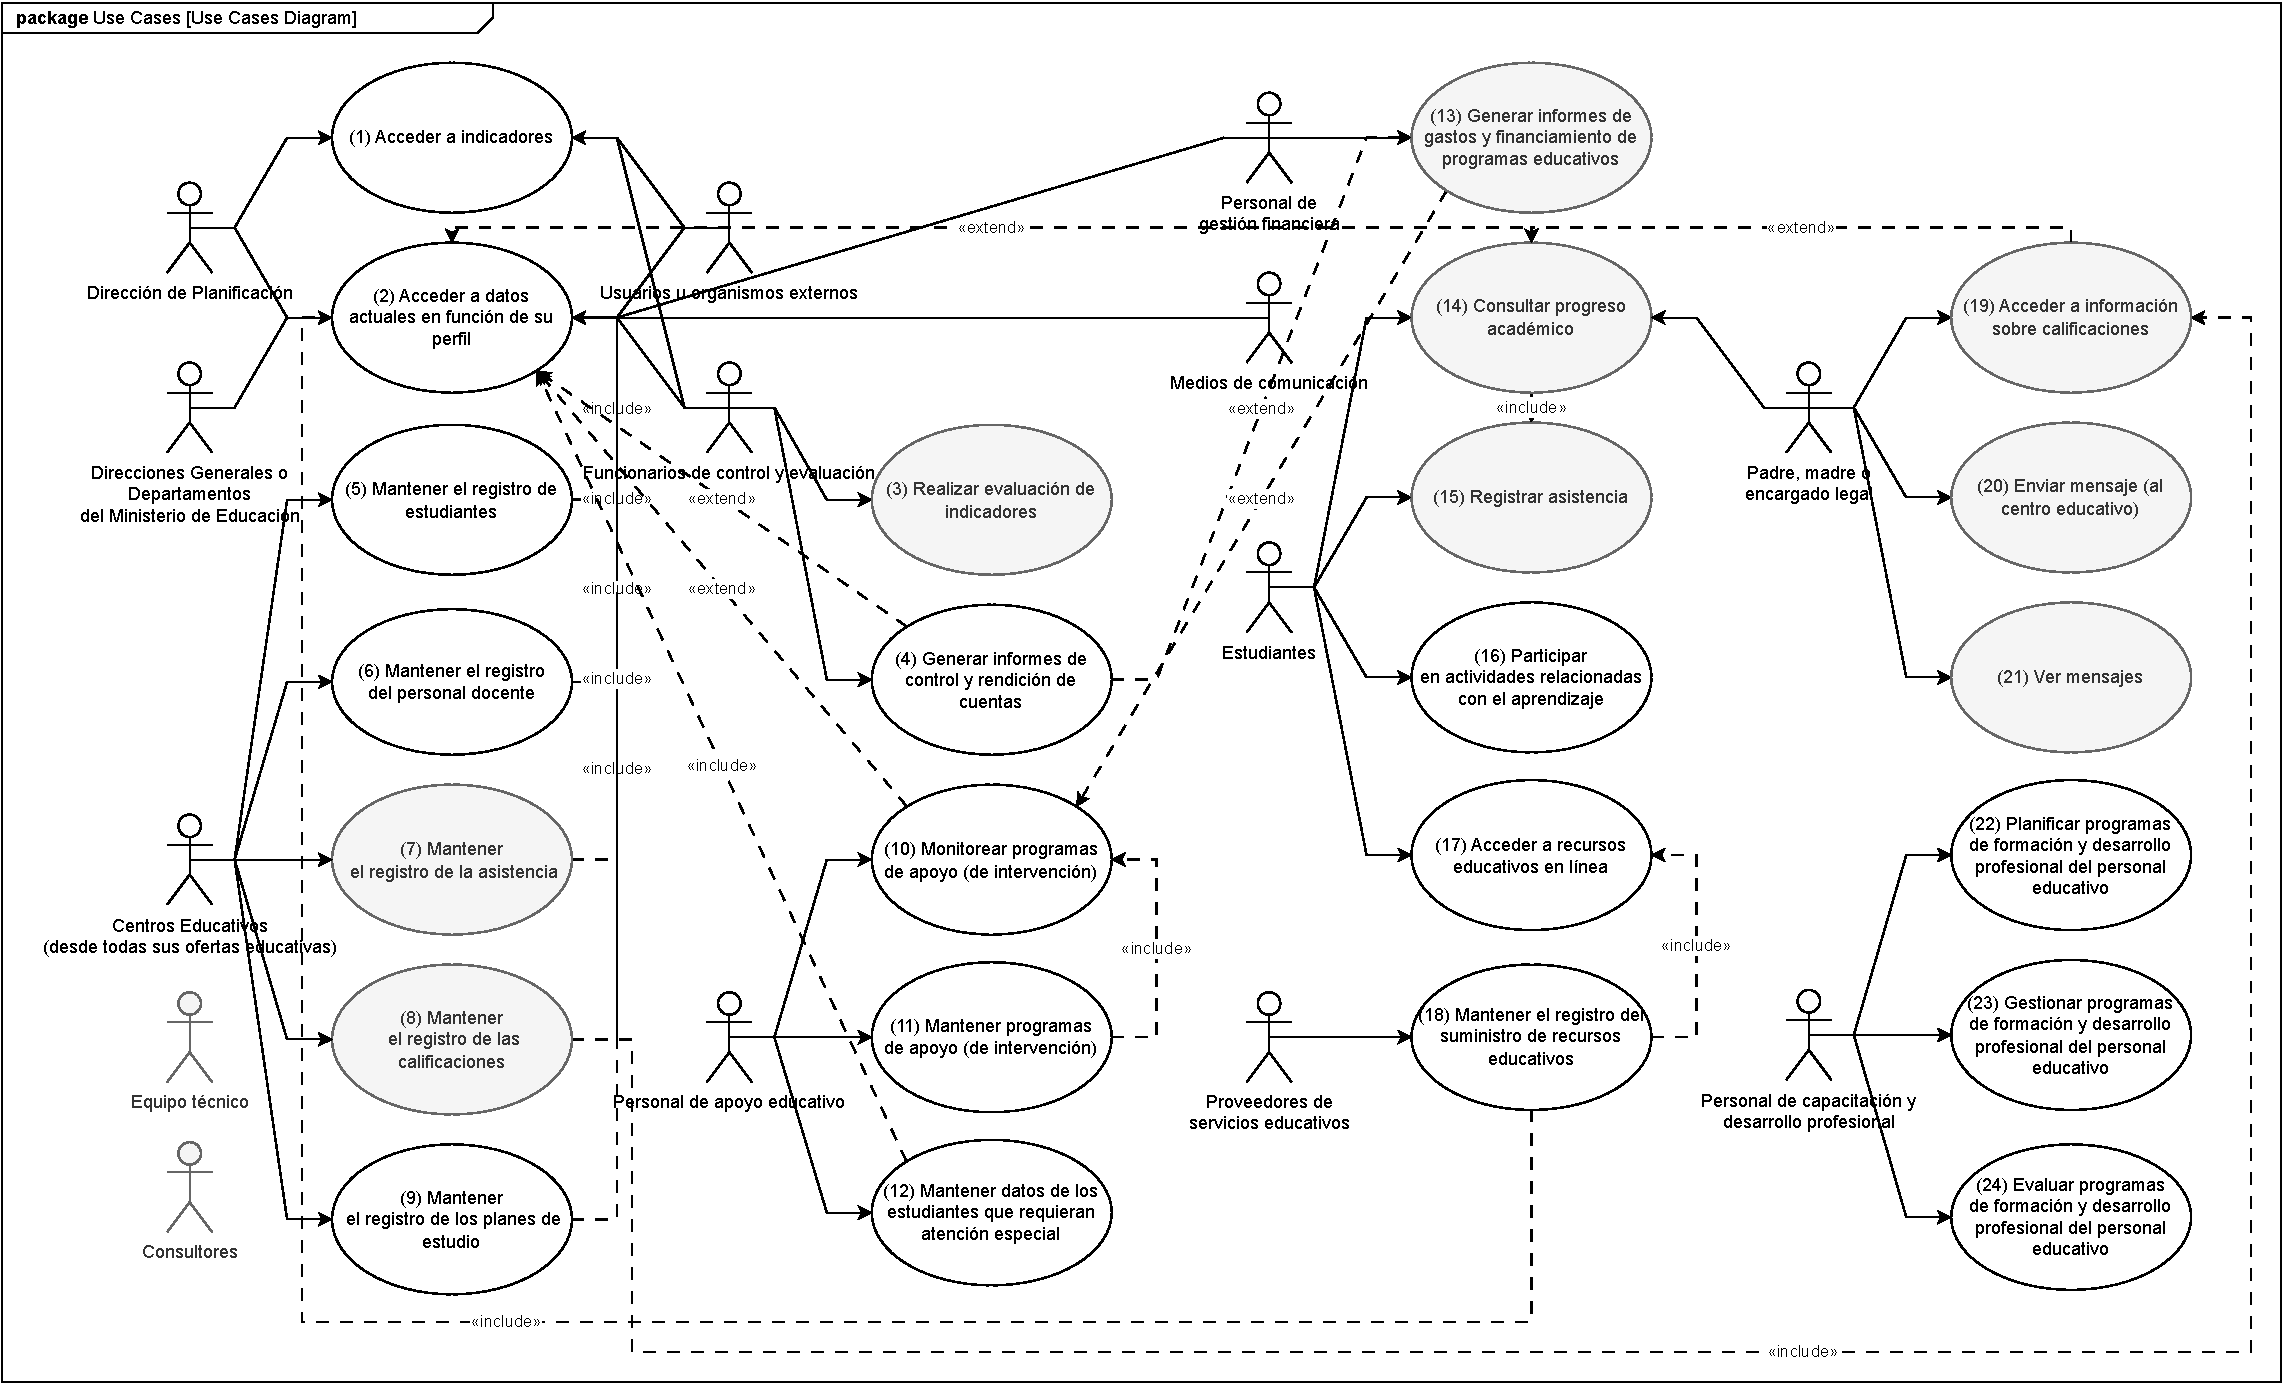
\includegraphics[width=\linewidth]{use} 
	\captionof{figure}{Diagrama de casos de uso. Cada monigote representa a un actor, y cada globo representa a un caso de uso. El conjunto de actores no se corresponde con el conjunto de entidades en el organigrama del ministerio. En el cuadro \ref{squ:workers}, a cada caso de uso se asigna un encargado que s\'i corresponde a una entidad en el organigrama del ministerio. Cada caso de uso de mantenimiento incluye las acciones ``cargar'', ``leer'', ``actualizar'' y ``eliminar''.}
	\label{fig:use}
 
 	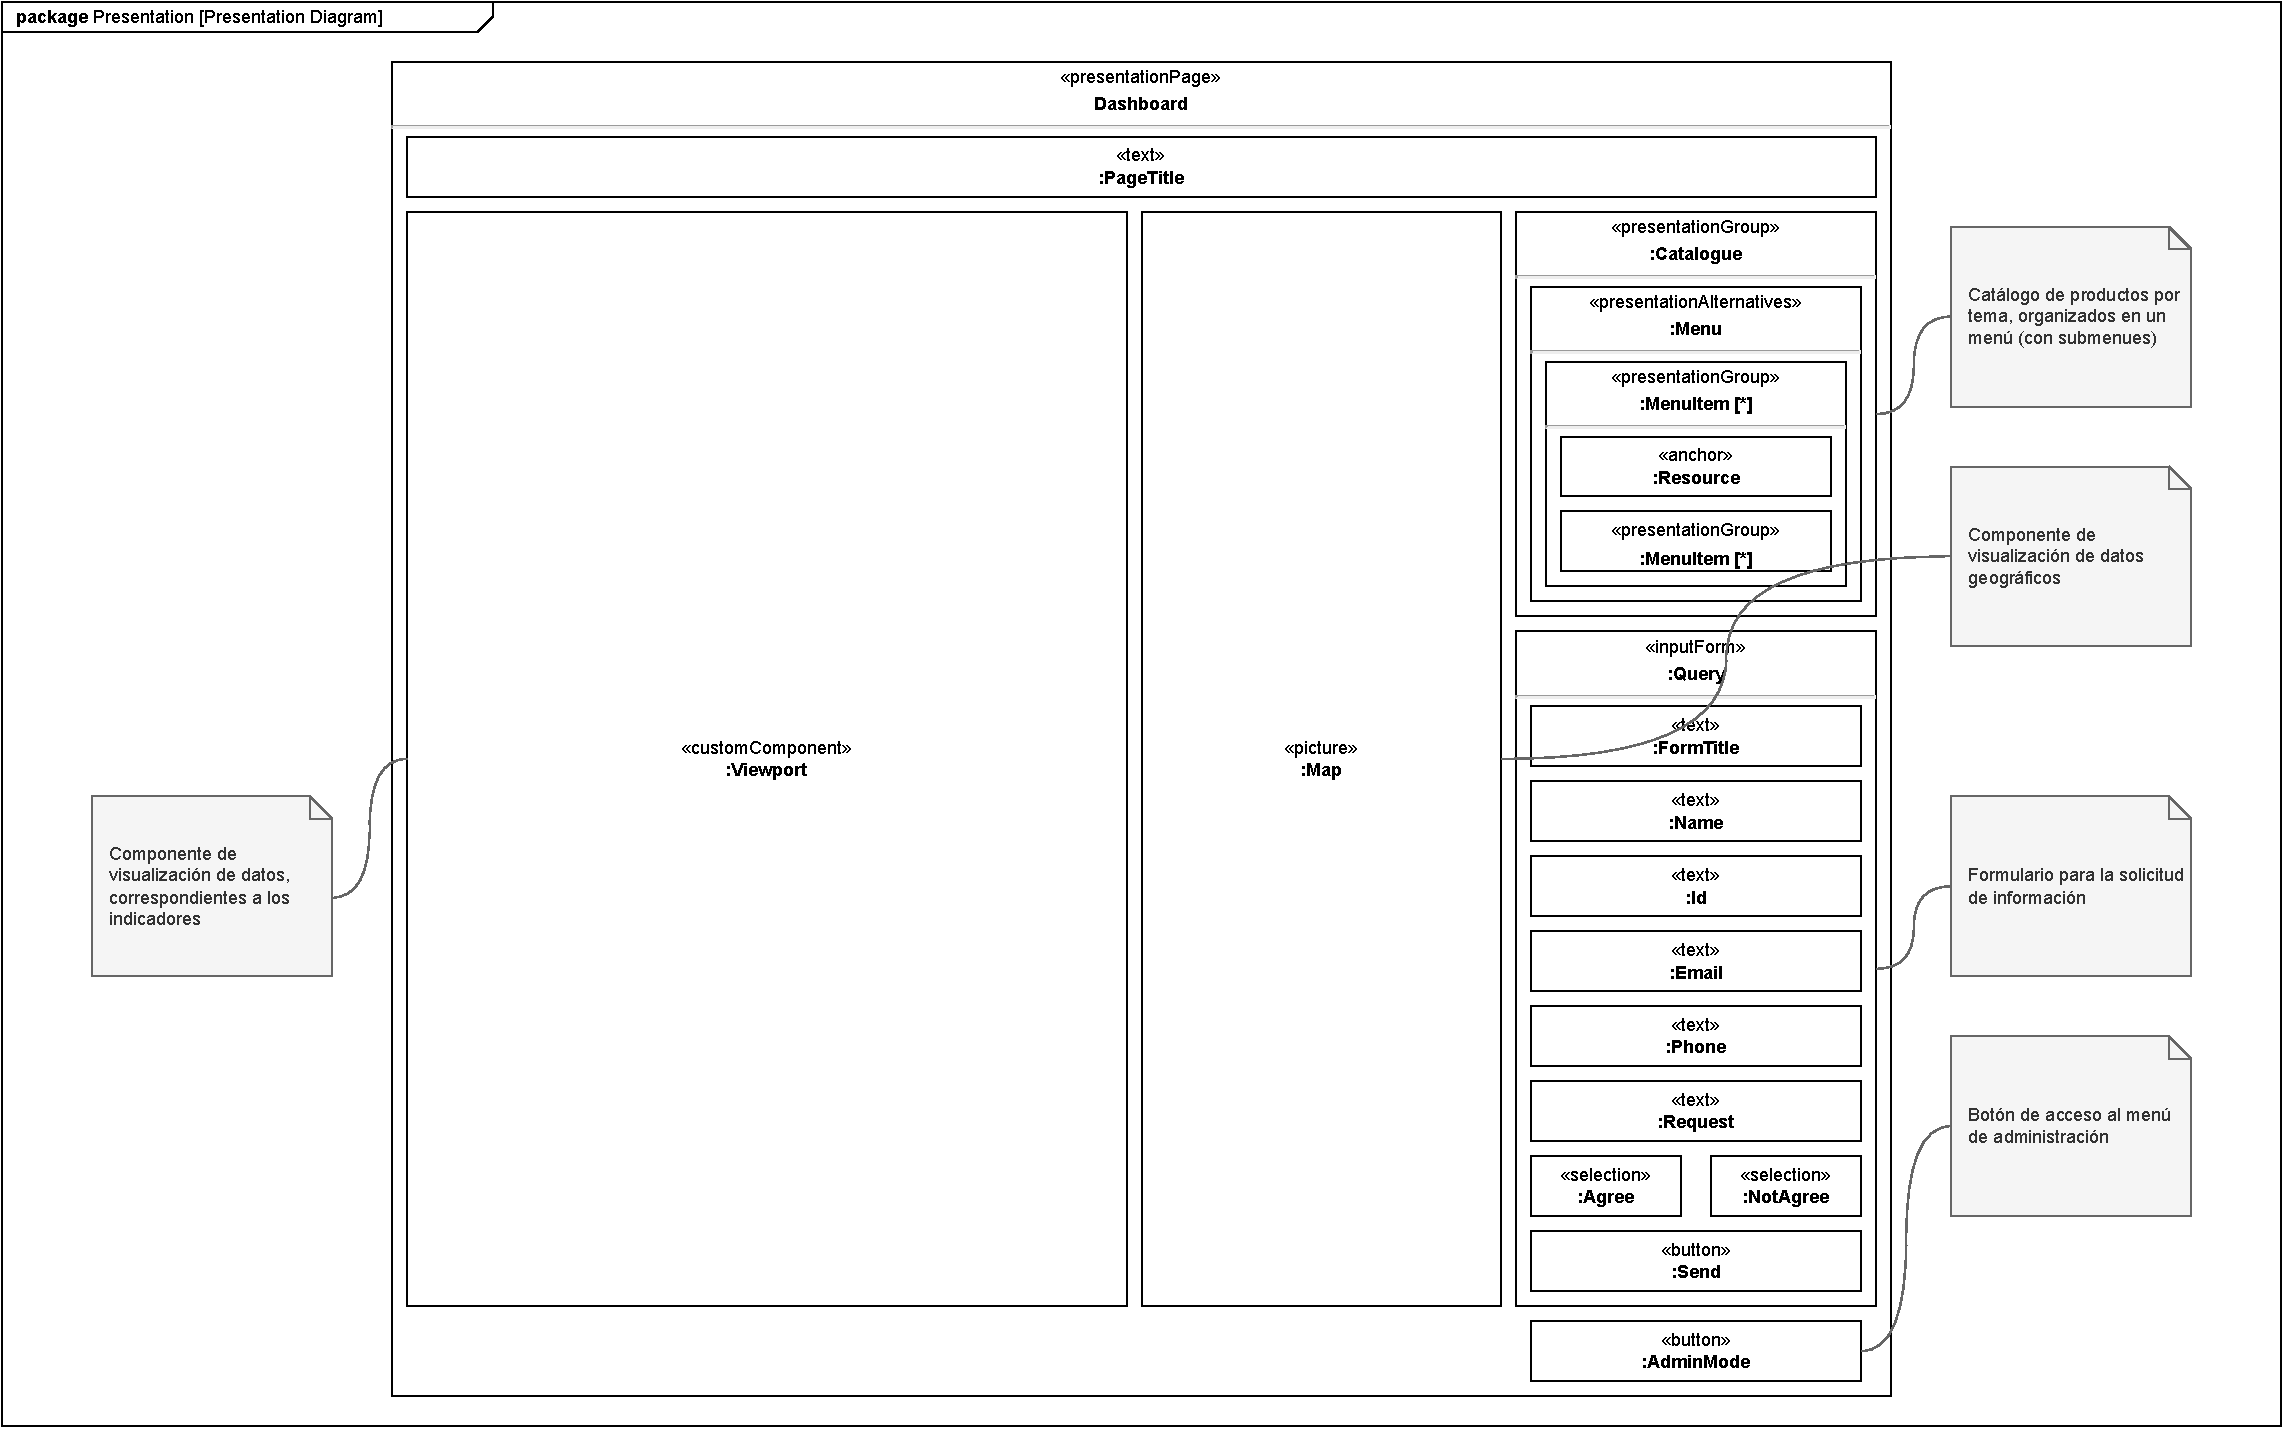
\includegraphics[width=\linewidth]{dashboard} 
 	\captionof{figure}{Diagrama presentaci\'on de la p\'agina de bienvenida.}
 	\label{fig:dash}
\end{minipage}%
\hspace{0.005\textwidth}
\begin{minipage}[b]{.685\textwidth}
 	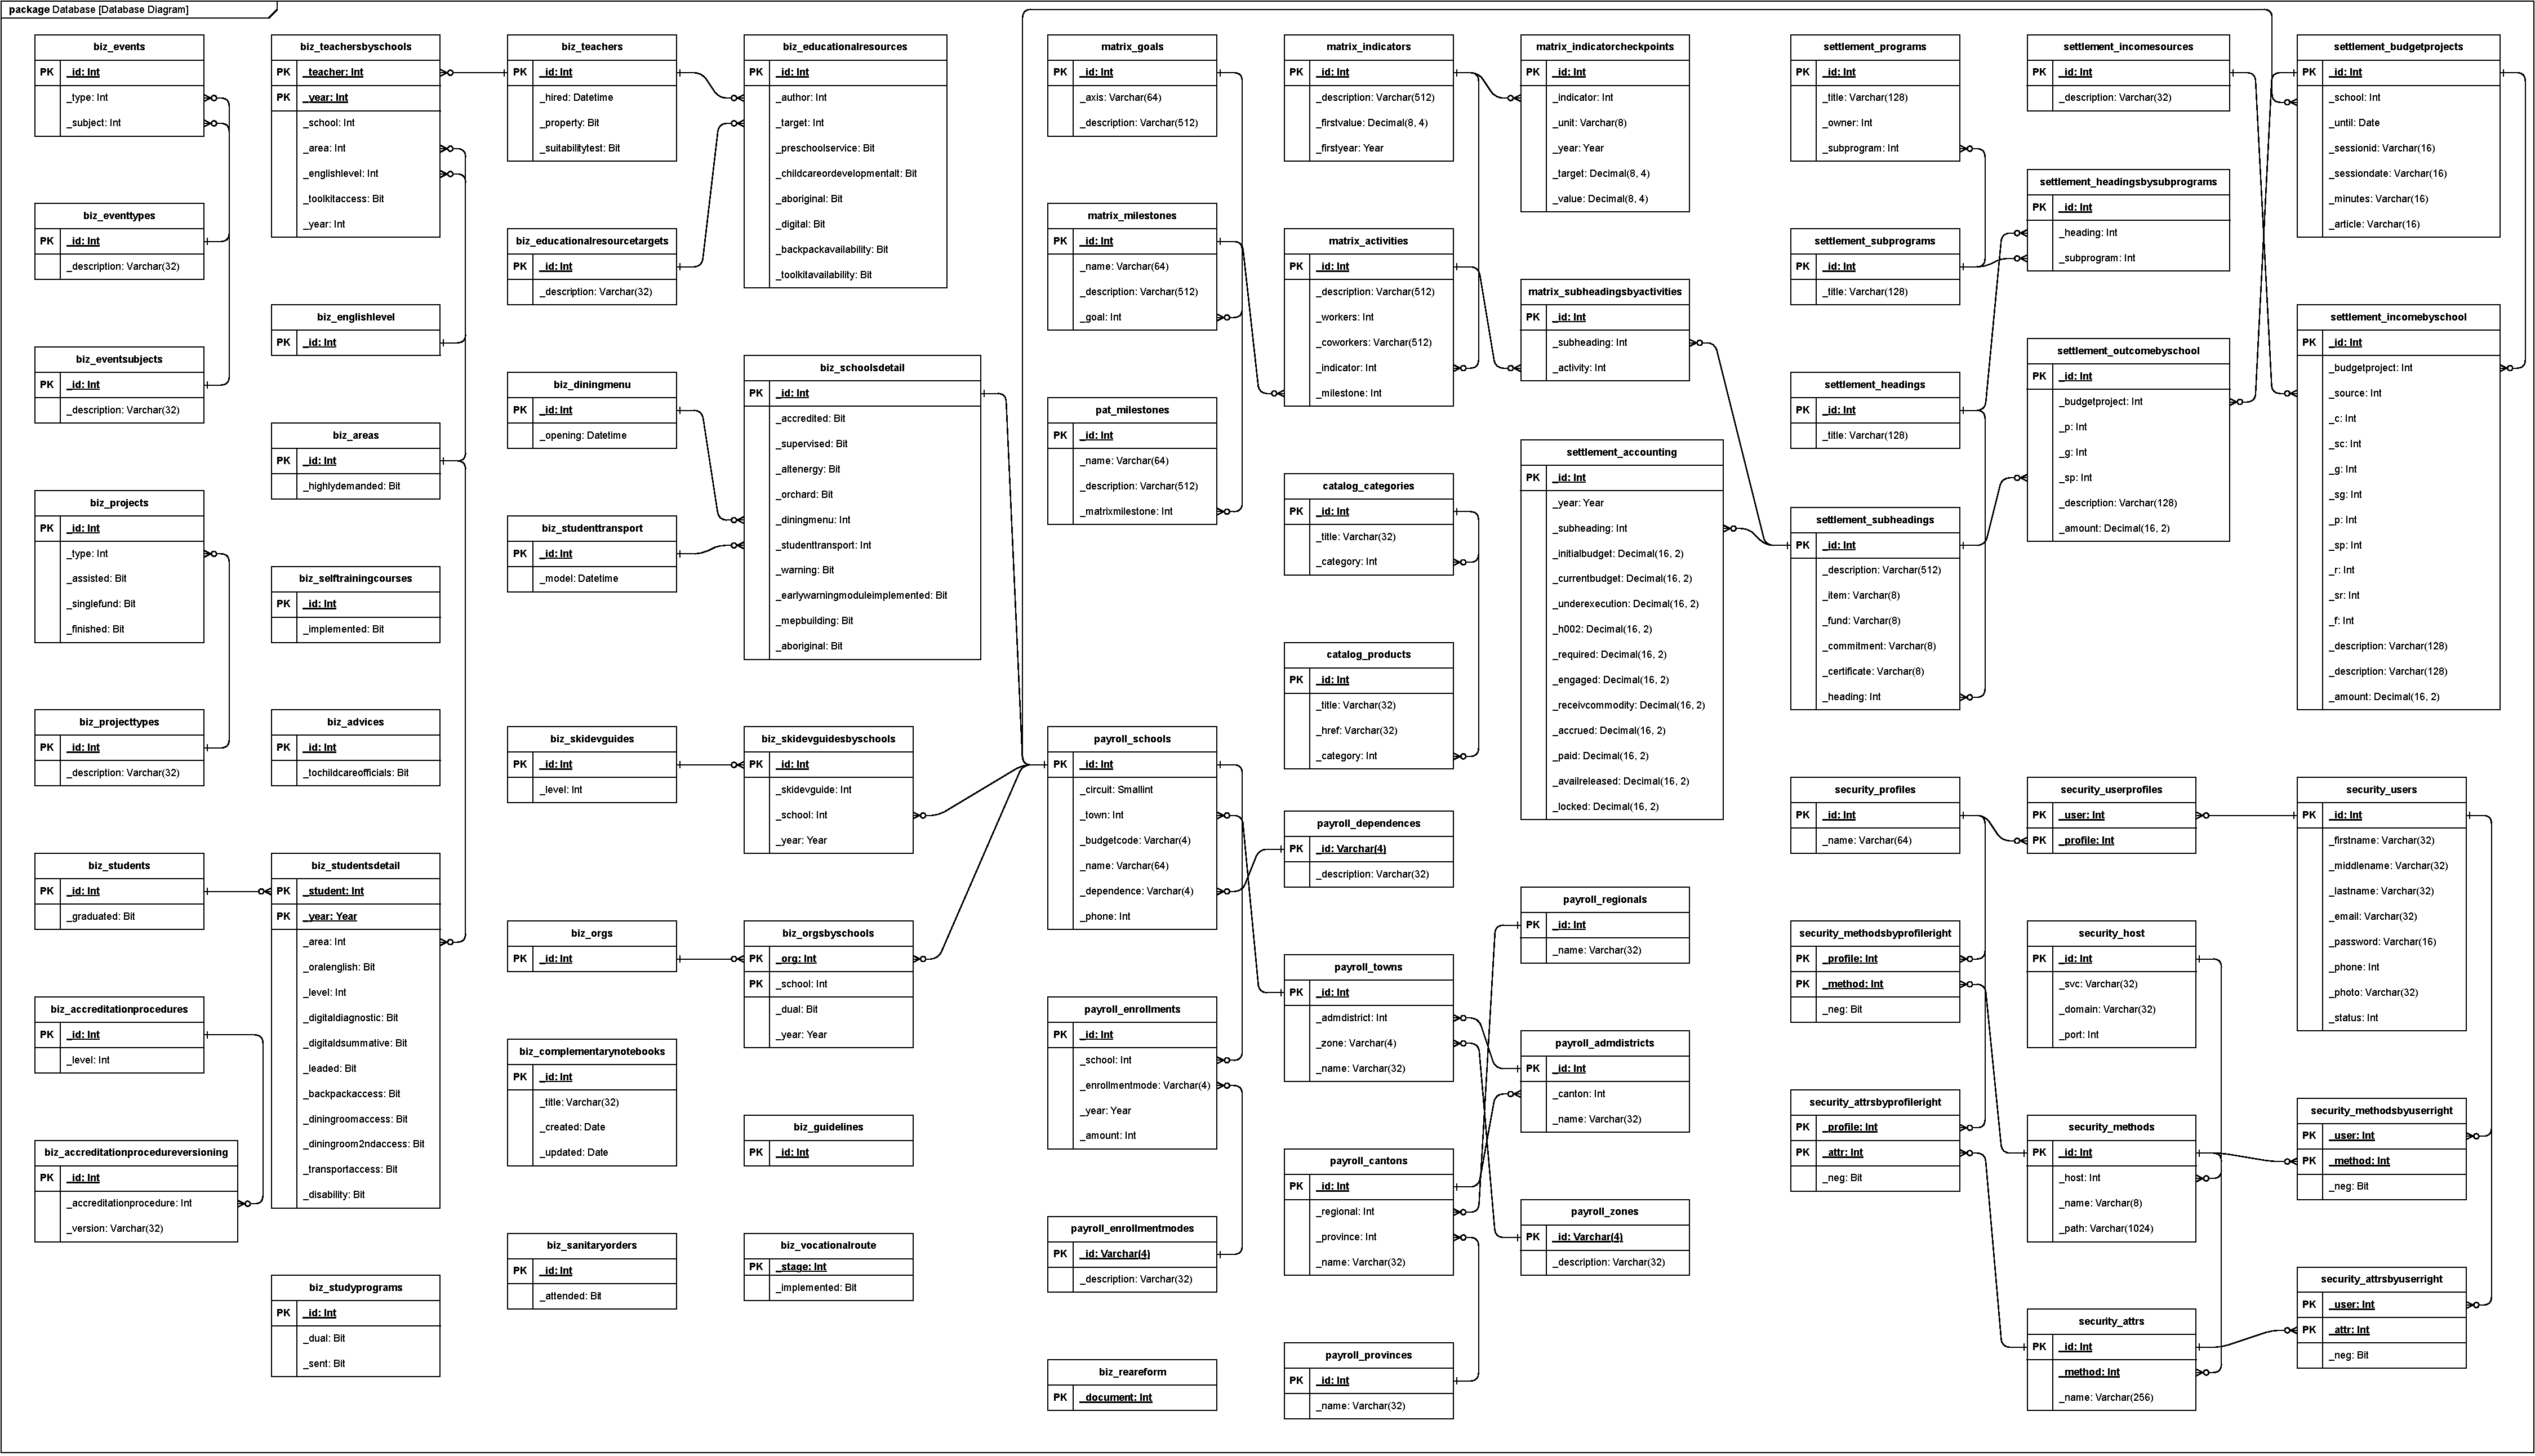
\includegraphics[width=\linewidth]{rem} 
 	\captionof{figure}{Diagrama de base de datos. Las tablas con prefijo ``payroll\_'', ``settlement\_'', ``matrix\_'', ``pat\_'', ``security\_'', ``biz\_'' y ``catalog\_'' corresponden a los m\'odulos de n\'omina de centros educativos, reporte de la liquidaci\'on general, indicadores, plan anual de trabajo (de centros educativos), seguridad, l\'ogica de negocio, y cat\'alogo de productos, respectivamente.}
 	\label{fig:rem}
\end{minipage}

% --------------------------------------------------------------------------------------------------------------------------------
\appendix
%section{Sem\'antica}



% --------------------------------------------------------------------------------------------------------------------------------
\section{Matriz de actividades e indicadores, Ruta de la Educaci\'on} \label{sec:matrix}

\begin{wraptable}{l}{\linewidth}
	\centering
	%caption{Matriz de actividades e indicadores}
	\label{tab:matrix}
	\rowcolors{2}{gray!20}{gray!10}
	\begin{tabular}{p{0.025\linewidth}p{0.1\linewidth}p{0.025\linewidth}p{0.175\linewidth}p{0.1\linewidth}p{0.1\linewidth}p{0.025\linewidth}p{0.025\linewidth}p{0.1\linewidth}p{0.1\linewidth}p{0.025\linewidth}p{0.025\linewidth}p{0.025\linewidth}p{0.025\linewidth}p{0.025\linewidth}p{0.025\linewidth}}
	\rowcolor{gray!40}
	Prop\'osito - eje competencia & Objetivo estrat\'egico & N & Nombre del Hito/Resultado & Descripci\'on & Actividades & Casos de uso que favorecen la implementaci\'on & Responsables de Planificaci\'on & Factores cr\'iticos y entes internos cooperantes MEP que favorecen la implementaci\'on & Indicadores & A\~no base & L\'inea base & A\~no & Meta anual & A\~no 3 & Meta final \\
	%hline
	I & Mejorar las competencias en las personas estudiantes mediante ofertas educativas con curr\'iculo pertinente, mediaci\'on pedag\'ogica, docentes capacitados, y evaluaci\'on continua. & 1 & Desarrollo de competencias & \begin{tabular}[c]{@{}p{\linewidth}}Se comprende la competencia como la uni\'on de las habilidades, los conocimientos, las aptitudes y los valores para la resoluci\'on de problemas.\\ Se comprende una competencia como la capacidad de aplicar los conocimientos, junto con las destrezas y habilidades, para desempe\~nar una actividad profesional, de manera satisfactoria y en un contexto determinado.\end{tabular} & 01.01 Elaborar Gu\'ias para el Desarrollo de Competencias seg\'un el nivel educativo (Preescolar, I y II Ciclos, III Ciclo y Educaci\'on Diversificada y EPJA) & 17, 18 & DDC & \begin{tabular}[c]{@{}p{\linewidth}}IDP (webinarios y videos)\\ DGDR (Articulaci\'on de la parte regional con la acad\'emica)\\ DRE (para validaci\'on y si se requiere capacitar en los programas y apoyar en el proceso de capacitaci\'on y asesoramiento)\\ DVE\end{tabular} & Cantidad de Gu\'ias elaboradas para el desarrollo de competencias seg\'un el nivel educativo & 2022 & 0 & \begin{tabular}[c]{@{}p{\linewidth}}2023\\ 2024\\ 2025\end{tabular} & \begin{tabular}[c]{@{}p{\linewidth}}12\\ 8\\ 8\end{tabular} & 2026 & \begin{tabular}[c]{@{}p{\linewidth}}28\\ (acumulado)\end{tabular} \\
	I & Mejorar las competencias en las personas estudiantes mediante ofertas educativas con curr\'iculo pertinente, mediaci\'on pedag\'ogica, docentes capacitados, y evaluaci\'on continua. & 1 & Desarrollo de competencias & \begin{tabular}[c]{@{}p{\linewidth}}Se comprende la competencia como la uni\'on de las habilidades, los conocimientos, las aptitudes y los valores para la resoluci\'on de problemas.\\ Se comprende una competencia como la capacidad de aplicar los conocimientos, junto con las destrezas y habilidades, para desempe\~nar una actividad profesional, de manera satisfactoria y en un contexto determinado.\end{tabular} & 01.02 Aplicar las Gu\'ias para el Desarrollo de Competencias en el marco de los programas de estudio. & 17, 18 & \begin{tabular}[c]{@{}p{\linewidth}}DRE\\ DGDR\\ DDC\end{tabular} & (Verificaci\'on/seguimiento de la aplicaci\'on de las gu\'ias). (Seguimiento de que las DRE est\'en supervisando la aplicaci\'on de las gu\'ias). & Porcentaje de Centros Educativos aplicando las Gu\'ias de desarrollo de competencias. & 2022 & 0\% & \begin{tabular}[c]{@{}p{\linewidth}}2023\\ 2024\\ 2025\end{tabular} & \begin{tabular}[c]{@{}p{\linewidth}}100\%\\ 100\%\\ 100\%\end{tabular} & 2026 & 100\% \\
	I & Mejorar las competencias en las personas estudiantes mediante ofertas educativas con curr\'iculo pertinente, mediaci\'on pedag\'ogica, docentes capacitados, y evaluaci\'on continua. & 1 & Desarrollo de competencias & \begin{tabular}[c]{@{}p{\linewidth}}Se comprende la competencia como la uni\'on de las habilidades, los conocimientos, las aptitudes y los valores para la resoluci\'on de problemas.\\ Se comprende una competencia como la capacidad de aplicar los conocimientos, junto con las destrezas y habilidades, para desempe\~nar una actividad profesional, de manera satisfactoria y en un contexto determinado.\end{tabular} & 01.03 Actualizar los programas de estudio orient\'andolos al desarrollo de competencias & 9 & \begin{tabular}[c]{@{}p{\linewidth}}DDC\\ DETCE\end{tabular} & CSE & Porcentaje de avance en la propuesta de actualizaci\'on de los programas de estudios orient\'andolos al desarrollo de competencias. & 2022 & 0\% & \begin{tabular}[c]{@{}p{\linewidth}}2024\\ 2025\\ 2026\end{tabular} & \begin{tabular}[c]{@{}p{\linewidth}}33\%\\ 33\%\\ 34\%\end{tabular} & 2026 & 100\% \\
	I & Mejorar las competencias en las personas estudiantes mediante ofertas educativas con curr\'iculo pertinente, mediaci\'on pedag\'ogica, docentes capacitados, y evaluaci\'on continua. & 1 & Desarrollo de competencias & \begin{tabular}[c]{@{}p{\linewidth}}Se comprende la competencia como la uni\'on de las habilidades, los conocimientos, las aptitudes y los valores para la resoluci\'on de problemas.\\ Se comprende una competencia como la capacidad de aplicar los conocimientos, junto con las destrezas y habilidades, para desempe\~nar una actividad profesional, de manera satisfactoria y en un contexto determinado.\end{tabular} & 01.04 Implementar una oferta formativa para capacitar a docentes en el desarrollo de competencias & 22, 23, 24 & IDPUGS & \begin{tabular}[c]{@{}p{\linewidth}}Direcci\'on de Desarrollo Curricular (Expertos en contenido) \\ DRE (coordinaci\'on para ejecuci\'on)\\ Inform\'atica de gesti\'on (fortalecimiento de la plataforma y conectividad)\\ Direcci\'on de Vida Estudiantil (Colaboraci\'on en actividades propias de la instancia)\\ Viceministerio Acad\'emico.\\ DRTE\\ DPI (Contenido econ\'omico)\\ DAIC (Suscripci\'on de convenios, cooperaci\'on externa)\\ DETCE (Colaboraci\'on en los cursos \'o m\'odulos t\'ecnicos)\\ Disposiciones de las autoridades para establecer lineamientos referidos a los espacios destinados a la capacitaci\'on de docentes.\\ Aliados estrat\'egicos\end{tabular} & Porcentaje de la oferta formativa implementada & 2022 & 0\% & \begin{tabular}[c]{@{}p{\linewidth}}2024\\ 2025\\ 2026\end{tabular} & \begin{tabular}[c]{@{}p{\linewidth}}100\%\\ 100\%\\ 100\%\end{tabular} & 2026 & 100\% \\
	I & Mejorar las competencias en las personas estudiantes mediante ofertas educativas con curr\'iculo pertinente, mediaci\'on pedag\'ogica, docentes capacitados, y evaluaci\'on continua. & 1 & Desarrollo de competencias & \begin{tabular}[c]{@{}p{\linewidth}}Se comprende la competencia como la uni\'on de las habilidades, los conocimientos, las aptitudes y los valores para la resoluci\'on de problemas.\\ Se comprende una competencia como la capacidad de aplicar los conocimientos, junto con las destrezas y habilidades, para desempe\~nar una actividad profesional, de manera satisfactoria y en un contexto determinado.\end{tabular} & 01.05 Actualizar el Reglamento de Evaluaci\'on de los Aprendizajes (REA), referidos a la promoci\'on del estudiantado que cursa el primer a\~no de la Educaci\'on General B\'asica & & DDC & \begin{tabular}[c]{@{}p{\linewidth}}(Departamento de Evaluaci\'on de los Aprendizajes)\\ CSE\\ DPSC\\ Direcci\'on de Asuntos Jur\'idicos\end{tabular} & Porcentaje de actualizaci\'on del Reglamento de Evaluaci\'on de los Aprendizajes (REA). & 2022 & 0\% & 2023 & 100\% & 2023 & 100\% \\
	I & Mejorar las competencias en las personas estudiantes mediante ofertas educativas con curr\'iculo pertinente, mediaci\'on pedag\'ogica, docentes capacitados, y evaluaci\'on continua. & 1 & Desarrollo de competencias & \begin{tabular}[c]{@{}p{\linewidth}}Se comprende la competencia como la uni\'on de las habilidades, los conocimientos, las aptitudes y los valores para la resoluci\'on de problemas.\\ Se comprende una competencia como la capacidad de aplicar los conocimientos, junto con las destrezas y habilidades, para desempe\~nar una actividad profesional, de manera satisfactoria y en un contexto determinado.\end{tabular} & \begin{tabular}[c]{@{}p{\linewidth}}01.06 Implementar la ruta de la lectura y escritura con la participaci\'on de diversos actores del \'ambito educativo nacional.\\ (Diagn\'ostico nacional para conocer el nivel de lectoescritura del estudiantado de primaria y secundaria, Gu\'ia con orientaciones pedag\'ogicas para el personal docente, Generaci\'on de recursos did\'acticos para el aprendizaje, Campa\~na nacional de divulgaci\'on de buenas pr\'acticas de lectoescritura, utilizando diferentes medios. Desarrollo de eventos regionales que fomenten el amor y el inter\'es por la lectoescritura).\end{tabular} & 17, 18 & DDC & \begin{tabular}[c]{@{}p{\linewidth}}Despacho de la Ministra\\ IDP (Webinarios y recursos did\'acticos)\\ DRTE (Producci\'on de recursos y dise\~nos publicitarios, coordinaci\'on de esfuerzas para bibliotecas escolares)\\ DGDR (Colaboraci\'on en la implementaci\'on a lo interno de la DRE)\\ DPRP (Log\'istica y divulgaci\'on de la ruta)\\ Direcci\'on de Vida Estudiantil (Colaboraci\'on en actividades propias de la instancia). \\ DRE colaboran\\ (DPSC, DEPI, DAEED, DETCED y DEPJA)\\ DVE\\ DPRP\end{tabular} & Porcentaje de avance de la implementaci\'on de la ruta de lectura & 2022 & 0\% & \begin{tabular}[c]{@{}p{\linewidth}}2023\\ 2024\\ 2025\end{tabular} & \begin{tabular}[c]{@{}p{\linewidth}}25\%\\ 25\%\\ 25\%\\ 25\%\end{tabular} & 2026 & 100\% \\
	I & Mejorar las competencias en las personas estudiantes mediante ofertas educativas con curr\'iculo pertinente, mediaci\'on pedag\'ogica, docentes capacitados, y evaluaci\'on continua. & 1 & Desarrollo de competencias & \begin{tabular}[c]{@{}p{\linewidth}}Se comprende la competencia como la uni\'on de las habilidades, los conocimientos, las aptitudes y los valores para la resoluci\'on de problemas.\\ Se comprende una competencia como la capacidad de aplicar los conocimientos, junto con las destrezas y habilidades, para desempe\~nar una actividad profesional, de manera satisfactoria y en un contexto determinado.\end{tabular} & \begin{tabular}[c]{@{}p{\linewidth}}01.07 Dise\~nar y elaborar programas de estudio de las especialidades t\'ecnicas que se imparten en la Educaci\'on Diversificada.\\ \\ Pendiente nuevo dato por Pablo Masis\end{tabular} & 9 & DETCE & \begin{tabular}[c]{@{}p{\linewidth}}Despacho Ministerial \\ Viceministerio Acad\'emico\\ CSE\end{tabular} & Cantidad de programas de estudio elaborados y presentados ante el CSE. & 2022 & 0 & \begin{tabular}[c]{@{}p{\linewidth}}2023\\ 2024\end{tabular} & \begin{tabular}[c]{@{}p{\linewidth}}17\\ 20\end{tabular} & 2026 & 37 \\
	I & Mejorar las competencias en las personas estudiantes mediante ofertas educativas con curr\'iculo pertinente, mediaci\'on pedag\'ogica, docentes capacitados, y evaluaci\'on continua. & 1 & Desarrollo de competencias & \begin{tabular}[c]{@{}p{\linewidth}}Se comprende la competencia como la uni\'on de las habilidades, los conocimientos, las aptitudes y los valores para la resoluci\'on de problemas.\\ Se comprende una competencia como la capacidad de aplicar los conocimientos, junto con las destrezas y habilidades, para desempe\~nar una actividad profesional, de manera satisfactoria y en un contexto determinado.\end{tabular} & 01.08 Incrementar la competencia oral en ingl\'es a trav\'es de evaluaciones digitales & 17 & \begin{tabular}[c]{@{}p{\linewidth}}DDC \\ DVE\\ DRE\end{tabular} & \begin{tabular}[c]{@{}p{\linewidth}}DGDR (Coordinaci\'on de aplicaci\'on de pruebas). DRE organiza e implementa las pruebas en los CE. Se encarga de la log\'istica de la aplicaci\'on .\\ DGEC (Coordinaci\'on de aplicaci\'on de pruebas)\\ DAIC\end{tabular} & Cantidad de estudiantes evaluados en sus competencias orales en ingl\'es & 2022 & & \begin{tabular}[c]{@{}p{\linewidth}}2024\\ 2025\end{tabular} & \begin{tabular}[c]{@{}p{\linewidth}}730\\ (500 Secun.\\ 230 Primar.) c/a\~no\end{tabular} & & \\
	I & Mejorar las competencias en las personas estudiantes mediante ofertas educativas con curr\'iculo pertinente, mediaci\'on pedag\'ogica, docentes capacitados, y evaluaci\'on continua. & 1 & Desarrollo de competencias & \begin{tabular}[c]{@{}p{\linewidth}}Se comprende la competencia como la uni\'on de las habilidades, los conocimientos, las aptitudes y los valores para la resoluci\'on de problemas.\\ Se comprende una competencia como la capacidad de aplicar los conocimientos, junto con las destrezas y habilidades, para desempe\~nar una actividad profesional, de manera satisfactoria y en un contexto determinado.\end{tabular} & 01.09 - Implementar el modelo de educaci\'on dual en los CTP con apoyo de los sectores productivos de la Regi\'on & 22, 23, 24 & DETCE & \begin{tabular}[c]{@{}p{\linewidth}}Despacho Ministerial \\ Viceministerio Acad\'emico\\ CSE\end{tabular} & Cantidad de empresas participantes implementando CTP modalidad dual. & 2022 & 0 & \begin{tabular}[c]{@{}p{\linewidth}}2023\\ 2024\\ 2025\\ 2026\end{tabular} & 8 & 2026 & 32 \\
	I & Mejorar las competencias en las personas estudiantes mediante ofertas educativas con curr\'iculo pertinente, mediaci\'on pedag\'ogica, docentes capacitados, y evaluaci\'on continua. & 1 & Desarrollo de competencias & \begin{tabular}[c]{@{}p{\linewidth}}Se comprende la competencia como la uni\'on de las habilidades, los conocimientos, las aptitudes y los valores para la resoluci\'on de problemas.\\ Se comprende una competencia como la capacidad de aplicar los conocimientos, junto con las destrezas y habilidades, para desempe\~nar una actividad profesional, de manera satisfactoria y en un contexto determinado.\end{tabular} & 01.10 Implementar el modelo de educaci\'on dual en los CTP con apoyo de los sectores productivos de la Regi\'on & 22, 23, 24 & DETCE & \begin{tabular}[c]{@{}p{\linewidth}}Despacho Ministerial \\ Viceministerio Acad\'emico\\ CSE\end{tabular} & Cantidad de Programas de estudio modalidad dual elaborados y presentado al CSE & & & \begin{tabular}[c]{@{}p{\linewidth}}2023\\ 2024\\ 2025\\ 2026\end{tabular} & 2 & 2026 & 11 \\
	I & Mejorar las competencias en las personas estudiantes mediante ofertas educativas con curr\'iculo pertinente, mediaci\'on pedag\'ogica, docentes capacitados, y evaluaci\'on continua. & 1 & Desarrollo de competencias & \begin{tabular}[c]{@{}p{\linewidth}}Se comprende la competencia como la uni\'on de las habilidades, los conocimientos, las aptitudes y los valores para la resoluci\'on de problemas.\\ Se comprende una competencia como la capacidad de aplicar los conocimientos, junto con las destrezas y habilidades, para desempe\~nar una actividad profesional, de manera satisfactoria y en un contexto determinado.\end{tabular} & 01.11 Certificar de manera gratuita a docentes en \'areas de mayor demanda laboral por parte de los sectores productivos de la Regi\'on & 22, 23, 24 & DETCE & \begin{tabular}[c]{@{}p{\linewidth}}Viceministerio Acad\'emico\\ DGEC\\ CAP\\ DETCE\\ DRTE\end{tabular} & Cantidad de docentes certificados en \'areas de mayor demanda laboral. & & & & & & \\
	I & Mejorar las competencias en las personas estudiantes mediante ofertas educativas con curr\'iculo pertinente, mediaci\'on pedag\'ogica, docentes capacitados, y evaluaci\'on continua. & 1 & Desarrollo de competencias & \begin{tabular}[c]{@{}p{\linewidth}}Se comprende la competencia como la uni\'on de las habilidades, los conocimientos, las aptitudes y los valores para la resoluci\'on de problemas.\\ Se comprende una competencia como la capacidad de aplicar los conocimientos, junto con las destrezas y habilidades, para desempe\~nar una actividad profesional, de manera satisfactoria y en un contexto determinado.\end{tabular} & 01.12 Certificar de manera gratuita a estudiantes en \'areas de mayor demanda laboral por parte de los sectores productivos de la Regi\'on & 16, 18 & DETCE & \begin{tabular}[c]{@{}p{\linewidth}}Viceministerio Acad\'emico\\ DGEC\\ CAP\\ DETCE\\ DRTE\end{tabular} & Cantidad de estudiantes certificados en \'areas de mayor demanda laboral. & & & & & & \\
	I & Mejorar las competencias en las personas estudiantes mediante ofertas educativas con curr\'iculo pertinente, mediaci\'on pedag\'ogica, docentes capacitados, y evaluaci\'on continua. & 1 & Desarrollo de competencias & \begin{tabular}[c]{@{}p{\linewidth}}Se comprende la competencia como la uni\'on de las habilidades, los conocimientos, las aptitudes y los valores para la resoluci\'on de problemas.\\ Se comprende una competencia como la capacidad de aplicar los conocimientos, junto con las destrezas y habilidades, para desempe\~nar una actividad profesional, de manera satisfactoria y en un contexto determinado.\end{tabular} & 01.13 Dise\~nar e implementar una estrategia de biling\"uismo para ampliar la cobertura de un segundo idioma en los centros educativos de preescolar (primera infancia). & & Despacho Acad\'emico & \begin{tabular}[c]{@{}p{\linewidth}}Viceministerio Acad\'emico (Manuel Rojas Mata)\\ DRTE\\ DETCE\\ Direcci\'on de Vida Estudiantil\end{tabular} & Cantidad de centros educativos que cuentan con docentes de ingl\'es en C1 & & \begin{tabular}[c]{@{}p{\linewidth}}19.9\% Preescolar\\ \\ 90\% primaria\end{tabular} & & & & \begin{tabular}[c]{@{}p{\linewidth}}4\% Pree incremento\\ \\ 4\% primaria\end{tabular} \\
	I & Mejorar las competencias en las personas estudiantes mediante ofertas educativas con curr\'iculo pertinente, mediaci\'on pedag\'ogica, docentes capacitados, y evaluaci\'on continua. & 2 & Robustecimiento de la calidad pedag\'ogica & Brindar recursos y materiales did\'acticos en diferentes formatos como apoyo al proceso de ense\~nanza y aprendizaje & 02.01 Elaborar, asesorar y acompa\~nar a docentes recursos pedag\'ogicos para el desarrollo de competencias, did\'actica disruptiva para mejorar la mediaci\'on pedag\'ogica y lograr la recuperaci\'on de los aprendizajes a estudiantes & 22, 23, 24 & \begin{tabular}[c]{@{}p{\linewidth}}DDC\\ DRE\end{tabular} & \begin{tabular}[c]{@{}p{\linewidth}}IDP (Dise\~no de actividades)\\ DAIC (Cooperaci\'on externa)\\ DRE/DAP asesora y acompa\~nan a los (as) docentes en el proceso mediante el PFP.\\ DVE\end{tabular} & Cantidad de recursos pedag\'ogicos elaborados & 2022 & 0 & \begin{tabular}[c]{@{}p{\linewidth}}2023\\ 2024\\ 2025\end{tabular} & \begin{tabular}[c]{@{}p{\linewidth}}10\\ 10\\ 10\end{tabular} & 2026 & 30 (acumulado) \\
	I & Mejorar las competencias en las personas estudiantes mediante ofertas educativas con curr\'iculo pertinente, mediaci\'on pedag\'ogica, docentes capacitados, y evaluaci\'on continua. & 2 & Robustecimiento de la calidad pedag\'ogica & Brindar recursos y materiales did\'acticos en diferentes formatos como apoyo al proceso de ense\~nanza y aprendizaje & 02.02 Actualizaci\'on del documento "L\'ineas de acci\'on para los servicios de apoyo educativo que se brindan desde la educaci\'on especial" (estrategia docencia compartida) & 11 & DDC & \begin{tabular}[c]{@{}p{\linewidth}}DGDR (Seguimiento a la Implementaci\'on)\\ IDP (Realizaci\'on de webinarios) DRE mediante las asesor\'ias regionales de Educaci\'on Especial brindan el acompa\~namiento y seguimiento de las l\'ineas de acci\'on. - brindar acompa\~namiento a docentes en las l\'ineas de acci\'on -\\ DPRP (Divulgaci\'on de Campa\~nas)\\ (Departamento de Apoyos Educativos para el estudiantado con discapacidad)\end{tabular} & \begin{tabular}[c]{@{}p{\linewidth}}DDC - Cantidad de documentos actualizados\\ \\ DRE - Porcentaje de acompa\~namientos realizados a docentes de servicios de apoyo en relaci\'on con las l\'ineas de acci\'on (meta 100\% por a\~no de solicitudes atendidas)\end{tabular} & 2022 & 1 & 2023 & 1 & 2026 & 3 \\
	I & Mejorar las competencias en las personas estudiantes mediante ofertas educativas con curr\'iculo pertinente, mediaci\'on pedag\'ogica, docentes capacitados, y evaluaci\'on continua. & 2 & Robustecimiento de la calidad pedag\'ogica & Brindar recursos y materiales did\'acticos en diferentes formatos como apoyo al proceso de ense\~nanza y aprendizaje & 02.03 Divulgar el documento "L\'ineas de acci\'on para los servicios de apoyo educativo que se brindan desde la educaci\'on especial", mediante campa\~nas. & 11 & DDC & \begin{tabular}[c]{@{}p{\linewidth}}DGDR (Seguimiento a la Implementaci\'on)\\ IDP (Realizaci\'on de webinarios) DRE mediante las asesor\'ias regionales de Educaci\'on Especial brindan el acompa\~namiento de las l\'ineas de acci\'on.\\ DPRP (Divulgaci\'on de Campa\~nas)\\ (Departamento de Apoyos Educativos para el estudiantado con discapacidad)\end{tabular} & \begin{tabular}[c]{@{}p{\linewidth}}Cantidad de campa\~nas de divulgaci\'on sobre los documentos elaborados\\ \\ DRE - Porcentaje de acompa\~namientos realizados a docentes de servicios de apoyo en relaci\'on con las l\'ineas de acci\'on (meta 100\% por a\~no de solicitudes atendidas)\end{tabular} & 2022 & 1 & 2023 & 1 & 2026 & 1 \\
	I & Mejorar las competencias en las personas estudiantes mediante ofertas educativas con curr\'iculo pertinente, mediaci\'on pedag\'ogica, docentes capacitados, y evaluaci\'on continua. & 2 & Robustecimiento de la calidad pedag\'ogica & Brindar recursos y materiales did\'acticos en diferentes formatos como apoyo al proceso de ense\~nanza y aprendizaje & 02.04 Actualizar los cuadernos complementarios \#1, \#2 y \#3 & 11 & \begin{tabular}[c]{@{}p{\linewidth}}DDC \\ DRE\end{tabular} & \begin{tabular}[c]{@{}p{\linewidth}}DGDR (Seguimiento a la Implementaci\'on)\\ IDP (Realizaci\'on de webinarios)\\ DRE mediante las asesor\'ias regionales de Educaci\'on Especial brindan el acompa\~namiento y seguimiento de las l\'ineas de acci\'on.\\ DPRP (Divulgaci\'on de Campa\~nas)\\ (Departamento de Apoyos Educativos para el estudiantado con discapacidad)\end{tabular} & \begin{tabular}[c]{@{}p{\linewidth}}Cantidad de cuadernos complementarios actualizados\\ \\ DRE - Porcentaje de acompa\~namientos realizados a docentes de servicios de apoyo en relaci\'on con las l\'ineas de acci\'on (meta 100\% por a\~no de solicitudes atendidas)\end{tabular} & 2022 & 3 & \begin{tabular}[c]{@{}p{\linewidth}}2023\\ 2024\\ 2025\end{tabular} & \begin{tabular}[c]{@{}p{\linewidth}}3\\ 3\\ 3\end{tabular} & 2026 & 9 \\
	I & Mejorar las competencias en las personas estudiantes mediante ofertas educativas con curr\'iculo pertinente, mediaci\'on pedag\'ogica, docentes capacitados, y evaluaci\'on continua. & 2 & Robustecimiento de la calidad pedag\'ogica & Brindar recursos y materiales did\'acticos en diferentes formatos como apoyo al proceso de ense\~nanza y aprendizaje & 02.05 Elaborar cinco cuadernos complementarios (discapacidad m\'ultiple, discapacidad intelectual, audici\'on y lenguaje, terapia del lenguaje y problemas de aprendizaje) & 11 & \begin{tabular}[c]{@{}p{\linewidth}}DDC \\ DRE\end{tabular} & \begin{tabular}[c]{@{}p{\linewidth}}DGDR (Seguimiento a la Implementaci\'on)\\ IDP (Realizaci\'on de webinarios) DRE mediante las asesor\'ias regionales de Educaci\'on Especial brindan el acompa\~namiento y seguimiento de las l\'ineas de acci\'on.\\ DPRP (Divulgaci\'on de Campa\~nas)\\ (Departamento de Apoyos Educativos para el estudiantado con discapacidad)\end{tabular} & \begin{tabular}[c]{@{}p{\linewidth}}Cantidad de cuadernos complementarios elaborados\\ \\ DRE - Porcentaje de acompa\~namientos realizados a docentes de servicios de apoyo en relaci\'on con las l\'ineas de acci\'on (meta 100\% por a\~no de solicitudes atendidas)\end{tabular} & 2022 & 0 & \begin{tabular}[c]{@{}p{\linewidth}}2023\\ 2024\\ 2025\end{tabular} & \begin{tabular}[c]{@{}p{\linewidth}}2\\ 1 \\ 2\end{tabular} & 2026 & 5 \\
	I & Mejorar las competencias en las personas estudiantes mediante ofertas educativas con curr\'iculo pertinente, mediaci\'on pedag\'ogica, docentes capacitados, y evaluaci\'on continua. & 2 & Robustecimiento de la calidad pedag\'ogica & Brindar recursos y materiales did\'acticos en diferentes formatos como apoyo al proceso de ense\~nanza y aprendizaje & 02.06 Elaborar una estrategia de divulgaci\'on de los cuadernos complementarios & & \begin{tabular}[c]{@{}p{\linewidth}}DDC \\ DRE\end{tabular} & \begin{tabular}[c]{@{}p{\linewidth}}DGDR (Seguimiento a la Implementaci\'on)\\ IDP (Realizaci\'on de webinarios) DRE mediante las asesor\'ias regionales de Educaci\'on Especial brindan el acompa\~namiento y seguimiento de las l\'ineas de acci\'on.\\ DPRP (Divulgaci\'on de Campa\~nas)\\ (Departamento de Apoyos Educativos para el estudiantado con discapacidad)\end{tabular} & \begin{tabular}[c]{@{}p{\linewidth}}Cantidad de estrategias de divulgaci\'on de cuadernos complementarios\\ \\ DRE - Porcentaje de acompa\~namientos realizados a docentes de servicios de apoyo en relaci\'on con las l\'ineas de acci\'on (meta 100\% por a\~no de solicitudes atendidas)\end{tabular} & 2022 & 0 & \begin{tabular}[c]{@{}p{\linewidth}}2023\\ 2024\\ 2025\end{tabular} & \begin{tabular}[c]{@{}p{\linewidth}}4\\ 2 \\ 2\end{tabular} & 2026 & 8 \\
	I & Mejorar las competencias en las personas estudiantes mediante ofertas educativas con curr\'iculo pertinente, mediaci\'on pedag\'ogica, docentes capacitados, y evaluaci\'on continua. & 2 & Robustecimiento de la calidad pedag\'ogica & Brindar recursos y materiales did\'acticos en diferentes formatos como apoyo al proceso de ense\~nanza y aprendizaje & \begin{tabular}[c]{@{}p{\linewidth}}02.07 Elaboraci\'on del Modelo Pedag\'ogico para centros de educaci\'on especial basado en competencias, que los preparen para la plena inclusi\'on social, laboral entre otros.\\ \\ I Etapa: Elaboraci\'on de propuesta\\ II Etapa: Consulta de diferentes instancias\\ III Etapa: Informe de resultados\\ IV Etapa: Validaci\'on\\ V Etapa: Presentaci\'on de la propuesta\end{tabular} & 11 & DDC & \begin{tabular}[c]{@{}p{\linewidth}}DGDR (Validaci\'on en las DRE). \\ DRE Participar en los procesos de construcci\'on y validaci\'on\\ CSE\\ Despacho Acad\'emico\end{tabular} & Porcentaje de avance del modelo pedag\'ogico para centros de educaci\'on especial & \begin{tabular}[c]{@{}p{\linewidth}}2022\\ 2023\end{tabular} & 100\% & \begin{tabular}[c]{@{}p{\linewidth}}2023\\ 2024\\ 2025\\ \\ 2023\\ 2024\\ 2025\\ 2026\end{tabular} & \begin{tabular}[c]{@{}p{\linewidth}}50\%\\ 50\%\\ 100\%\\ \\ I, II y III Etapa\\ IV y V Etapa\\ Implementaci\'on \\ Seguimiento\end{tabular} & 2026 & 100\% \\
	I & Mejorar las competencias en las personas estudiantes mediante ofertas educativas con curr\'iculo pertinente, mediaci\'on pedag\'ogica, docentes capacitados, y evaluaci\'on continua. & 2 & Robustecimiento de la calidad pedag\'ogica & Brindar recursos y materiales did\'acticos en diferentes formatos como apoyo al proceso de ense\~nanza y aprendizaje & 02.08 Implementar la estrategia de Educaci\'on Intercultural. & 22, 23, 24 & DDC & \begin{tabular}[c]{@{}p{\linewidth}}DIE \\ DGDR (Validaci\'on en las DRE). \\ DRE - comunicaci\'on de casos, participaci\'on de campa\~nas y jornadas de trabajo con asesores nacionales Direcci\'on de Vida Estudiantil\\ (Departamento de Educaci\'on Intercultural)\end{tabular} & Porcentaje de avance de la implementaci\'on de la Estrategia & 2022 & 0\% & \begin{tabular}[c]{@{}p{\linewidth}}2023\\ 2024\\ 2025\\ 2026\end{tabular} & \begin{tabular}[c]{@{}p{\linewidth}}25\%\\ 25\%\\ 25\%\\ 25\%\end{tabular} & 2026 & 100\% \\
	I & Mejorar las competencias en las personas estudiantes mediante ofertas educativas con curr\'iculo pertinente, mediaci\'on pedag\'ogica, docentes capacitados, y evaluaci\'on continua. & 2 & Robustecimiento de la calidad pedag\'ogica & Brindar recursos y materiales did\'acticos en diferentes formatos como apoyo al proceso de ense\~nanza y aprendizaje & 02.09 Dise\~nar e implementar la ruta vocacional & 9, 22, 23, 24 & DVE & \begin{tabular}[c]{@{}p{\linewidth}}DDC\\ DRE (seguimiento de la ruta vocacional)\\ DGDR\end{tabular} & Cantidad de etapas implementadas de la ruta vocacional & 2022 & 0 & \begin{tabular}[c]{@{}p{\linewidth}}2023\\ 2024\\ 2025\end{tabular} & \begin{tabular}[c]{@{}p{\linewidth}}1\\ 1\\ 1\end{tabular} & 2025 & 3 \\
	I & Mejorar las competencias en las personas estudiantes mediante ofertas educativas con curr\'iculo pertinente, mediaci\'on pedag\'ogica, docentes capacitados, y evaluaci\'on continua. & 4 & Evaluaci\'on Estandarizada digital para calidad educativa & La evaluaci\'on de los aprendizajes, es un proceso continuo de recopilaci\'on de informaci\'on cualitativa y cuantitativa, que fundamenta la emisi\'on de juicios de valor y la toma de decisiones por parte de la persona docente y el estudiantado, para la mejora progresiva de los procesos de ense\~nanza y aprendizaje. & 04.01 Aplicar la Prueba Nacional Estandarizada Digital diagn\'ostica & 18 & \begin{tabular}[c]{@{}p{\linewidth}}DGEC\\ DRTE\end{tabular} & \begin{tabular}[c]{@{}p{\linewidth}}DIG. \\ DGDR\\ DRE (colaboran en la log\'istica, el desarrollo e implementaci\'on de las pruebas)\end{tabular} & Porcentaje de estudiantes que aplican las pruebas diagn\'osticas en forma digital. & 2023 & 0\% & \begin{tabular}[c]{@{}p{\linewidth}}2023\\ 2024\\ 2025\end{tabular} & \begin{tabular}[c]{@{}p{\linewidth}}100\%\\ 100\%\\ 100\%\end{tabular} & & \\
	I & Mejorar las competencias en las personas estudiantes mediante ofertas educativas con curr\'iculo pertinente, mediaci\'on pedag\'ogica, docentes capacitados, y evaluaci\'on continua. & 4 & Evaluaci\'on Estandarizada digital para calidad educativa & La evaluaci\'on de los aprendizajes, es un proceso continuo de recopilaci\'on de informaci\'on cualitativa y cuantitativa, que fundamenta la emisi\'on de juicios de valor y la toma de decisiones por parte de la persona docente y el estudiantado, para la mejora progresiva de los procesos de ense\~nanza y aprendizaje. & 04.02 Aplicar la Prueba Nacional Estandarizada Digital sumativa. & 18 & \begin{tabular}[c]{@{}p{\linewidth}}DGEC\\ DRTE\end{tabular} & \begin{tabular}[c]{@{}p{\linewidth}}DIG. \\ DRE (colabora con log\'istica, el desarrollo e implementaci\'on de las pruebas)\end{tabular} & Porcentaje de estudiantes que aplican las pruebas sumativas en forma digital. & 2023 & 0\% & \begin{tabular}[c]{@{}p{\linewidth}}2023\\ 2024\\ 2025\end{tabular} & \begin{tabular}[c]{@{}p{\linewidth}}100\%\\ 100\%\\ 100\%\end{tabular} & & \\
	I & Mejorar las competencias en las personas estudiantes mediante ofertas educativas con curr\'iculo pertinente, mediaci\'on pedag\'ogica, docentes capacitados, y evaluaci\'on continua. & 4 & Evaluaci\'on Estandarizada digital para calidad educativa & La evaluaci\'on de los aprendizajes, es un proceso continuo de recopilaci\'on de informaci\'on cualitativa y cuantitativa, que fundamenta la emisi\'on de juicios de valor y la toma de decisiones por parte de la persona docente y el estudiantado, para la mejora progresiva de los procesos de ense\~nanza y aprendizaje. & 04.03 Dise\~nar cursos de autoformaci\'on para acceder a la prueba digital de obtenci\'on del t\'itulo de bachillerato & & DDC & \begin{tabular}[c]{@{}p{\linewidth}}UPRE: Criterio para dirigir acciones a las personas que fueron excluidas del sistema educativo y requieren reincorporarse\\ DIG\\ Despacho ministerial (docentes destacados)\end{tabular} & Cantidad de cursos dise\~nados & 2022 & 1 & \begin{tabular}[c]{@{}p{\linewidth}}2023\\ 2024\end{tabular} & \begin{tabular}[c]{@{}p{\linewidth}}2\\ 4\end{tabular} & 2025 & 6 \\
	I & Mejorar las competencias en las personas estudiantes mediante ofertas educativas con curr\'iculo pertinente, mediaci\'on pedag\'ogica, docentes capacitados, y evaluaci\'on continua. & 4 & Evaluaci\'on Estandarizada digital para calidad educativa & La evaluaci\'on de los aprendizajes, es un proceso continuo de recopilaci\'on de informaci\'on cualitativa y cuantitativa, que fundamenta la emisi\'on de juicios de valor y la toma de decisiones por parte de la persona docente y el estudiantado, para la mejora progresiva de los procesos de ense\~nanza y aprendizaje. & 04.04 Implementar cursos de autoformaci\'on para acceder a la prueba digital de obtenci\'on del t\'itulo de bachillerato & 18 & DDC & \begin{tabular}[c]{@{}p{\linewidth}}UPRE: Criterio para dirigir acciones a las personas que fueron excluidas del sistema educativo y requieren reincorporarse\\ DIG\\ Despacho ministerial (docentes destacados)\end{tabular} & Cantidad de cursos implementados & & & \begin{tabular}[c]{@{}p{\linewidth}}2024\\ 2025\end{tabular} & \begin{tabular}[c]{@{}p{\linewidth}}2\\ 4\end{tabular} & 2026 & 6 \\
	I & Mejorar las competencias en las personas estudiantes mediante ofertas educativas con curr\'iculo pertinente, mediaci\'on pedag\'ogica, docentes capacitados, y evaluaci\'on continua. & 4 & Evaluaci\'on Estandarizada digital para calidad educativa & La evaluaci\'on de los aprendizajes, es un proceso continuo de recopilaci\'on de informaci\'on cualitativa y cuantitativa, que fundamenta la emisi\'on de juicios de valor y la toma de decisiones por parte de la persona docente y el estudiantado, para la mejora progresiva de los procesos de ense\~nanza y aprendizaje. & 04.05 Implementar un Bachillerato para la Empleabilidad mediante la colaboraci\'on con la Universidad Estatal a Distancia de Costa Rica. & 18 & DGEC & \begin{tabular}[c]{@{}p{\linewidth}}UPRE: Criterio para dirigir acciones a las personas que fueron excluidas del sistema educativo y requieren reincorporarse\\ DDC: Departamentos de j\'ovenes y adultos DGDR\\ DRE (colaboraci\'on divulgar informaci\'on a estudiantes rezagados)\end{tabular} & Porcentaje de avance para la implementaci\'on del Bachillerato para la Empleabilidad & & & 2023 & 100\% & & \\
	I & Mejorar las competencias en las personas estudiantes mediante ofertas educativas con curr\'iculo pertinente, mediaci\'on pedag\'ogica, docentes capacitados, y evaluaci\'on continua. & 4 & Evaluaci\'on Estandarizada digital para calidad educativa & La evaluaci\'on de los aprendizajes, es un proceso continuo de recopilaci\'on de informaci\'on cualitativa y cuantitativa, que fundamenta la emisi\'on de juicios de valor y la toma de decisiones por parte de la persona docente y el estudiantado, para la mejora progresiva de los procesos de ense\~nanza y aprendizaje. & 04.06 Implementar el Sistema de Gesti\'on de la Calidad Educativa & & DGEC & \begin{tabular}[c]{@{}p{\linewidth}}DGDR\\ DRE (vinculaci\'on con centros educativos)\\ UPRE: Criterio para dirigir acciones a las personas que fueron excluidas del sistema educativo y requieren reincorporarse\\ Comisi\'on Nacional de la Calidad\\ CSE\\ IDPUGS\end{tabular} & Porcentaje de avance en la implementaci\'on del Sistema de Acreditaci\'on de Calidad Educativa & 2022 & 0\% & \begin{tabular}[c]{@{}p{\linewidth}}2023\\ 2024\end{tabular} & \begin{tabular}[c]{@{}p{\linewidth}}50\%\\ 50\%\end{tabular} & 2026 & 100\% \\
	\end{tabular}
\end{wraptable}

\begin{wraptable}{l}{\linewidth}
	\centering
	\rowcolors{2}{gray!20}{gray!10}
	\begin{tabular}{p{0.025\linewidth}p{0.1\linewidth}p{0.025\linewidth}p{0.175\linewidth}p{0.1\linewidth}p{0.1\linewidth}p{0.025\linewidth}p{0.025\linewidth}p{0.1\linewidth}p{0.1\linewidth}p{0.025\linewidth}p{0.025\linewidth}p{0.025\linewidth}p{0.025\linewidth}p{0.025\linewidth}p{0.025\linewidth}}
	\rowcolor{gray!40}
	Prop\'osito - eje competencia & Objetivo estrat\'egico & N & Nombre del hito/Resultado & Descripci\'on & Actividades & Casos de uso que favorecen la implementaci\'on & Responsables de planificaci\'on & Factores cr\'iticos y entes internos cooperantes MEP que favorecen la implementaci\'on & Indicadores & A\~no base & L\'inea base & A\~no & Meta anual & A\~no 3 & Meta final \\
	%hline
	I & Mejorar las competencias en las personas estudiantes mediante ofertas educativas con curr\'iculo pertinente, mediaci\'on pedag\'ogica, docentes capacitados, y evaluaci\'on continua. & 5 & Evaluaci\'on de los aprendizajes del aula & Para desarrollar estrategias de recuperaci\'on de los aprendizajes en el aula y verificar el avance en el desempe\~no a estudiantes, docentes a nivel nacional aplicar\'an una prueba comprensiva para orientar la Recuperaci\'on de los Aprendizajes o Figuras Afines al inicio, se aplicar\'an al inicio del curso lectivo, a partir del 27 de febrero y la segunda, a partir del 31 de julio. a docentes deben realizar un diagn\'ostico donde se corrobore el nivel de preparaci\'on a estudiantes, conforme al Reglamento de Evaluaci\'on de los Aprendizajes recientemente aprobado por el CSE (AC-CSE-19-03-2023), que establece que las funciones de la evaluaci\'on de los aprendizajes permite conocer el estado inicial del estudiante en las \'areas del desarrollo: cognoscitiva, socio afectiva y psicomotriz; con base en la informaci\'on obtenida, permite la aplicaci\'on de estrategias para la recuperaci\'on de aprendizajes. & 05.01 Elaboraci\'on de la reforma integral al Reglamento de Evaluaci\'on de los Aprendizajes (REA) & & DDC & \begin{tabular}[c]{@{}p{\linewidth}}Viceministerio Acad\'emico DRE (para proceso de consulta y validaci\'on de la reforma)\\ DGDR\end{tabular} & Cantidad de documentos & 2022 & 0 & 2023 & 1 & 2023 & 1 \\
	I & Mejorar las competencias en las personas estudiantes mediante ofertas educativas con curr\'iculo pertinente, mediaci\'on pedag\'ogica, docentes capacitados, y evaluaci\'on continua. & 5 & Evaluaci\'on de los aprendizajes del aula & Para desarrollar estrategias de recuperaci\'on de los aprendizajes en el aula y verificar el avance en el desempe\~no a estudiantes, docentes a nivel nacional aplicar\'an una prueba comprensiva para orientar la Recuperaci\'on de los Aprendizajes o Figuras Afines al inicio, se aplicar\'an al inicio del curso lectivo, a partir del 27 de febrero y la segunda, a partir del 31 de julio. a docentes deben realizar un diagn\'ostico donde se corrobore el nivel de preparaci\'on a estudiantes, conforme al Reglamento de Evaluaci\'on de los Aprendizajes recientemente aprobado por el CSE (AC-CSE-19-03-2023), que establece que las funciones de la evaluaci\'on de los aprendizajes permite conocer el estado inicial del estudiante en las \'areas del desarrollo: cognoscitiva, socio afectiva y psicomotriz; con base en la informaci\'on obtenida, permite la aplicaci\'on de estrategias para la recuperaci\'on de aprendizajes. & 05.02 Elaborar los lineamientos t\'ecnicos para la implementaci\'on y aplicaci\'on de las Pruebas comprensivas & & DDC & \begin{tabular}[c]{@{}p{\linewidth}}Viceministerio Acad\'emico\\ DRE (para proceso de consulta y validaci\'on de la reforma)\\ DGDR\end{tabular} & Cantidad de lineamientos t\'ecnicos referidos a las Pruebas comprensivas. & 2022 & 0 & \begin{tabular}[c]{@{}p{\linewidth}}2023\\ 2024\\ 2025\end{tabular} & \begin{tabular}[c]{@{}p{\linewidth}}2\\ 1\\ 1\end{tabular} & 2026 & 4 \\
	I & Mejorar las competencias en las personas estudiantes mediante ofertas educativas con curr\'iculo pertinente, mediaci\'on pedag\'ogica, docentes capacitados, y evaluaci\'on continua. & 5 & Evaluaci\'on de los aprendizajes del aula & Para desarrollar estrategias de recuperaci\'on de los aprendizajes en el aula y verificar el avance en el desempe\~no a estudiantes, docentes a nivel nacional aplicar\'an una prueba comprensiva para orientar la Recuperaci\'on de los Aprendizajes o Figuras Afines al inicio, se aplicar\'an al inicio del curso lectivo, a partir del 27 de febrero y la segunda, a partir del 31 de julio. a docentes deben realizar un diagn\'ostico donde se corrobore el nivel de preparaci\'on a estudiantes, conforme al Reglamento de Evaluaci\'on de los Aprendizajes recientemente aprobado por el CSE (AC-CSE-19-03-2023), que establece que las funciones de la evaluaci\'on de los aprendizajes permite conocer el estado inicial del estudiante en las \'areas del desarrollo: cognoscitiva, socio afectiva y psicomotriz; con base en la informaci\'on obtenida, permite la aplicaci\'on de estrategias para la recuperaci\'on de aprendizajes. & 05.03 Desarrollar acciones de acompa\~namiento y recuperaci\'on orientadas a la mejora de los aprendizajes a estudiantes a partir de la aplicaci\'on de las pruebas comprensivas & 18 & \begin{tabular}[c]{@{}p{\linewidth}}DRE\\ DIG\end{tabular} & \begin{tabular}[c]{@{}p{\linewidth}}Direcci\'on Curricular. DRE-C.E. (brindan acompa\~namiento t\'ecnico) UPRE: Alerta temprana, estudiantes en riesgo de exclusi\'on educativa\\ Direcci\'on de Inform\'atica de Gesti\'on \\ DGDR\end{tabular} & Porcentaje de estudiantes que se les aplica las acciones de acompa\~namiento. & & & 2023 & 100\% & & \\
	I & Mejorar las competencias en las personas estudiantes mediante ofertas educativas con curr\'iculo pertinente, mediaci\'on pedag\'ogica, docentes capacitados, y evaluaci\'on continua. & 5 & Evaluaci\'on de los aprendizajes del aula & Para desarrollar estrategias de recuperaci\'on de los aprendizajes en el aula y verificar el avance en el desempe\~no a estudiantes, docentes a nivel nacional aplicar\'an una prueba comprensiva para orientar la Recuperaci\'on de los Aprendizajes o Figuras Afines al inicio, se aplicar\'an al inicio del curso lectivo, a partir del 27 de febrero y la segunda, a partir del 31 de julio. a docentes deben realizar un diagn\'ostico donde se corrobore el nivel de preparaci\'on a estudiantes, conforme al Reglamento de Evaluaci\'on de los Aprendizajes recientemente aprobado por el CSE (AC-CSE-19-03-2023), que establece que las funciones de la evaluaci\'on de los aprendizajes permite conocer el estado inicial del estudiante en las \'areas del desarrollo: cognoscitiva, socio afectiva y psicomotriz; con base en la informaci\'on obtenida, permite la aplicaci\'on de estrategias para la recuperaci\'on de aprendizajes. & 05.04 Brindar asesoramiento a asesores regionales de evaluaci\'on mediante los asesores del nivel central & 22, 23 & DDC & \begin{tabular}[c]{@{}p{\linewidth}}DGDR (colaborar con la coordinaci\'on para las convocatorias)\\ DRE (Para la asistencia a las convocatorias)\end{tabular} & Cantidad de asesoramientos realizados & 2022 & 1 & \begin{tabular}[c]{@{}p{\linewidth}}2023\\ 2024\\ 2025\end{tabular} & \begin{tabular}[c]{@{}p{\linewidth}}1\\ 1\\ 1\end{tabular} & 2026 & \begin{tabular}[c]{@{}p{\linewidth}}3\\ (acumulado)\end{tabular} \\
	I & Mejorar las competencias en las personas estudiantes mediante ofertas educativas con curr\'iculo pertinente, mediaci\'on pedag\'ogica, docentes capacitados, y evaluaci\'on continua. & 5 & Evaluaci\'on de los aprendizajes del aula & Para desarrollar estrategias de recuperaci\'on de los aprendizajes en el aula y verificar el avance en el desempe\~no a estudiantes, docentes a nivel nacional aplicar\'an una prueba comprensiva para orientar la Recuperaci\'on de los Aprendizajes o Figuras Afines al inicio, se aplicar\'an al inicio del curso lectivo, a partir del 27 de febrero y la segunda, a partir del 31 de julio. a docentes deben realizar un diagn\'ostico donde se corrobore el nivel de preparaci\'on a estudiantes, conforme al Reglamento de Evaluaci\'on de los Aprendizajes recientemente aprobado por el CSE (AC-CSE-19-03-2023), que establece que las funciones de la evaluaci\'on de los aprendizajes permite conocer el estado inicial del estudiante en las \'areas del desarrollo: cognoscitiva, socio afectiva y psicomotriz; con base en la informaci\'on obtenida, permite la aplicaci\'on de estrategias para la recuperaci\'on de aprendizajes. & 05.05 Implementar el Sistema de Evaluaci\'on \'Agil (SEA), como apoyo a la labor docente en el proceso de evaluaci\'on de los aprendizajes & 18 & \begin{tabular}[c]{@{}p{\linewidth}}DIG\\ DGEC\end{tabular} & \begin{tabular}[c]{@{}p{\linewidth}}Direcci\'on Curricular (Aporta informaci\'on t\'ecnica bajo consultas realizadas de la instancia responsable)\\ DRE implementa el SEA y brinda el seguimiento de la aplicaci\'on en cada CE DRTE\\ DGDR\end{tabular} & Porcentaje de avance en la implementaci\'on del Sistema de Evaluaci\'on \'Agil (SEA) & & & 2023 & 100\% & & \\
	I & Mejorar las competencias en las personas estudiantes mediante ofertas educativas con curr\'iculo pertinente, mediaci\'on pedag\'ogica, docentes capacitados, y evaluaci\'on continua. & 6 & Desarrollo de aceleradores para la recuperaci\'on & \begin{tabular}[c]{@{}p{\linewidth}}Las personas estudiantes contar\'an con una Mochila Digital (en l\'inea y fuera de l\'inea) que contiene recursos did\'acticos para fortalecer y recuperar los aprendizajes. Esta se encontrar\'a disponible a partir del segundo semestre 2023 y se continuar\'a complementando y actualizando a lo largo de los a\~nos lectivos.\\ Todos a docentes contar\'an con la Caja de Herramientas, que contiene recursos did\'acticos actualizados y atractivos para mejorar el proceso de ense\~nanza, tambi\'en a mediados del 2023. Se promueve el uso de aceleradores que incluye juegos, actividades y din\'amicas que le ponen color, motivaci\'on, interactividad y alegr\'ia al aprendizaje.\\ Algunos de los aceleradores que ya est\'an producidos son:\\ $\bullet$ Programa STEAM \\ $\bullet$ Aprendo Pura Vida\\ $\bullet$ Plataforma Nacional Educativa \\ $\bullet$ Programa Nacional Leyendo y Contando producido en alianza con Microsoft C.R \\ $\bullet$ ABC Mouse\\ $\bullet$ My Math Academy\end{tabular} & 06.01 Elaborar un inventario de aceleradores disponibles en diversas plataformas para coordinar con la DDC el mapeo y correlaci\'on con la malla curricular. & 18 & DRTE & \begin{tabular}[c]{@{}p{\linewidth}}Direcci\'on de Vida Estudiantil \\ DGDR\\ UPRE: acciones dirigidas a estudiantes en riesgo de exclusi\'on educativa o que se reincorporan al estudio\\ La DRE mediante el DAP elabora estrategias, materiales y recursos.\\ DDC\end{tabular} & Porcentaje de recursos digitales y aceleradores disponibles en la mochila digital. & & & 2023 & 100\% & & \\
	I & Mejorar las competencias en las personas estudiantes mediante ofertas educativas con curr\'iculo pertinente, mediaci\'on pedag\'ogica, docentes capacitados, y evaluaci\'on continua. & 6 & Desarrollo de aceleradores para la recuperaci\'on & \begin{tabular}[c]{@{}p{\linewidth}}Las personas estudiantes contar\'an con una Mochila Digital (en l\'inea y fuera de l\'inea) que contiene recursos did\'acticos para fortalecer y recuperar los aprendizajes. Esta se encontrar\'a disponible a partir del segundo semestre 2023 y se continuar\'a complementando y actualizando a lo largo de los a\~nos lectivos.\\ Todos a docentes contar\'an con la Caja de Herramientas, que contiene recursos did\'acticos actualizados y atractivos para mejorar el proceso de ense\~nanza, tambi\'en a mediados del 2023. Se promueve el uso de aceleradores que incluye juegos, actividades y din\'amicas que le ponen color, motivaci\'on, interactividad y alegr\'ia al aprendizaje.\\ Algunos de los aceleradores que ya est\'an producidos son:\\ $\bullet$ Programa STEAM \\ $\bullet$ Aprendo Pura Vida\\ $\bullet$ Plataforma Nacional Educativa \\ $\bullet$ Programa Nacional Leyendo y Contando producido en alianza con Microsoft C.R \\ $\bullet$ ABC Mouse\\ $\bullet$ My Math Academy\end{tabular} & 06.02 Proporcionar al estudiantado el acceso a la "Mochila Digital" & 17 & DRTE & \begin{tabular}[c]{@{}p{\linewidth}}Direcci\'on de Vida Estudiantil \\ DGDR\\ UPRE: acciones dirigidas a estudiantes en riesgo de exclusi\'on educativa o que se reincorporan al estudio\\ La DRE mediante el DAP elabora estrategias, materiales y recursos.\\ DDC\end{tabular} & Cantidad de estudiantes beneficiados con el acceso a la "Mochila Digital" & & & \begin{tabular}[c]{@{}p{\linewidth}}2023\\ 2024\end{tabular} & \begin{tabular}[c]{@{}p{\linewidth}}300,000\\ 1,000,000\end{tabular} & & \\
	I & Mejorar las competencias en las personas estudiantes mediante ofertas educativas con curr\'iculo pertinente, mediaci\'on pedag\'ogica, docentes capacitados, y evaluaci\'on continua. & 6 & Desarrollo de aceleradores para la recuperaci\'on & \begin{tabular}[c]{@{}p{\linewidth}}Las personas estudiantes contar\'an con una Mochila Digital (en l\'inea y fuera de l\'inea) que contiene recursos did\'acticos para fortalecer y recuperar los aprendizajes. Esta se encontrar\'a disponible a partir del segundo semestre 2023 y se continuar\'a complementando y actualizando a lo largo de los a\~nos lectivos.\\ Todos a docentes contar\'an con la Caja de Herramientas, que contiene recursos did\'acticos actualizados y atractivos para mejorar el proceso de ense\~nanza, tambi\'en a mediados del 2023. Se promueve el uso de aceleradores que incluye juegos, actividades y din\'amicas que le ponen color, motivaci\'on, interactividad y alegr\'ia al aprendizaje.\\ Algunos de los aceleradores que ya est\'an producidos son:\\ $\bullet$ Programa STEAM \\ $\bullet$ Aprendo Pura Vida\\ $\bullet$ Plataforma Nacional Educativa \\ $\bullet$ Programa Nacional Leyendo y Contando producido en alianza con Microsoft C.R \\ $\bullet$ ABC Mouse\\ $\bullet$ My Math Academy\end{tabular} & 06.03 Elaborar un inventario de aceleradores disponibles en diversas plataformas para coordinar con la DDC, DGE y el IDP la correlaci\'on con las necesidades docentes. & 18 & DRTE & \begin{tabular}[c]{@{}p{\linewidth}}DRE\\ Direcci\'on de Vida Estudiantil \\ DGDR\\ DDC\end{tabular} & Porcentaje de recursos digitales y aceleradores disponibles en la caja de herramientas. & & & 2023 & 100\% & & \\
	I & Mejorar las competencias en las personas estudiantes mediante ofertas educativas con curr\'iculo pertinente, mediaci\'on pedag\'ogica, docentes capacitados, y evaluaci\'on continua. & 6 & Desarrollo de aceleradores para la recuperaci\'on & \begin{tabular}[c]{@{}p{\linewidth}}Las personas estudiantes contar\'an con una Mochila Digital (en l\'inea y fuera de l\'inea) que contiene recursos did\'acticos para fortalecer y recuperar los aprendizajes. Esta se encontrar\'a disponible a partir del segundo semestre 2023 y se continuar\'a complementando y actualizando a lo largo de los a\~nos lectivos.\\ Todos a docentes contar\'an con la Caja de Herramientas, que contiene recursos did\'acticos actualizados y atractivos para mejorar el proceso de ense\~nanza, tambi\'en a mediados del 2023. Se promueve el uso de aceleradores que incluye juegos, actividades y din\'amicas que le ponen color, motivaci\'on, interactividad y alegr\'ia al aprendizaje.\\ Algunos de los aceleradores que ya est\'an producidos son:\\ $\bullet$ Programa STEAM \\ $\bullet$ Aprendo Pura Vida\\ $\bullet$ Plataforma Nacional Educativa \\ $\bullet$ Programa Nacional Leyendo y Contando producido en alianza con Microsoft C.R \\ $\bullet$ ABC Mouse\\ $\bullet$ My Math Academy\end{tabular} & 06.04 Brindar acceso a docentes acceso a la "Caja de Herramientas" & & DRTE & \begin{tabular}[c]{@{}p{\linewidth}}DRE\\ Direcci\'on de Vida Estudiantil \\ DGDR\\ DDC\end{tabular} & Cantidad de docentes que acceden a la "Caja de Herramientas". & & & \begin{tabular}[c]{@{}p{\linewidth}}2023\\ 2024\end{tabular} & \begin{tabular}[c]{@{}p{\linewidth}}50,000\\ 30,000\end{tabular} & & \\
	I & Mejorar las competencias en las personas estudiantes mediante ofertas educativas con curr\'iculo pertinente, mediaci\'on pedag\'ogica, docentes capacitados, y evaluaci\'on continua. & 7 & Educaci\'on de primera infancia & Apoyo educativo que brindar\'a a los centros de cuido y desarrollo infantil a partir de la reforma de la Ley de Red Nacional de Cuido y Desarrollo Infantil liderada por la Segunda Vicepresidencia de la Rep\'ublica que coordina el sector social & 07.01 Brindar asesor\'ia t\'ecnico-curricular en los procesos pedag\'ogicos a las personas funcionarias de la atenci\'on de la ni\~nez en Alternativas de Cuido y Desarrollo Infantil. & 22, 23 & DDC & \begin{tabular}[c]{@{}p{\linewidth}}IDP (Para Realizaci\'on de Webinarios y talleres) \\ DGDR (coordinaci\'on y verificaci\'on con las DRE\\ DRE/DAP (mediante las Asesor\'ias de Preescolar coordina acciones y brinda seguimiento a los procesos)\\ UPRE: criterio para dirigir acciones a poblaciones en mayor riesgo y vulnerabilidad\\ DAEED\\ Comisi\'on Interna del MEP\end{tabular} & Cantidad de asesor\'ias brindadas a las personas funcionarias de la atenci\'on de la ni\~nez en Alternativas de Cuido y Desarrollo Infantil & 2022 & 2 & \begin{tabular}[c]{@{}p{\linewidth}}2023\\ 2024\\ 2025\end{tabular} & \begin{tabular}[c]{@{}p{\linewidth}}2\\ 2\\ 2\end{tabular} & 2026 & 6 \\
	I & Mejorar las competencias en las personas estudiantes mediante ofertas educativas con curr\'iculo pertinente, mediaci\'on pedag\'ogica, docentes capacitados, y evaluaci\'on continua. & 7 & Educaci\'on de primera infancia & Apoyo educativo que brindar\'a a los centros de cuido y desarrollo infantil a partir de la reforma de la Ley de Red Nacional de Cuido y Desarrollo Infantil liderada por la Segunda Vicepresidencia de la Rep\'ublica que coordina el sector social & 07.02 Registrar digitalmente a la poblaci\'on usuaria de los servicios de Educaci\'on Preescolar en las Alternativas de Cuido y Desarrollo Infantil p\'ublicas y privadas acreditadas. & 5 & \begin{tabular}[c]{@{}p{\linewidth}}DDC\\ DIG\\ DEP\end{tabular} & \begin{tabular}[c]{@{}p{\linewidth}}DIG (Saber) / DPI (Estad\'istica)\\ UPRE: Identificaci\'on de personas en riesgo o exclusi\'on mediante alerta temprana\\ CROE (Acreditaci\'on P\'ublicos externos MEP)\\ Centros Privados (Acreditaci\'on Privados)\\ DRE (asesor\'ia y fiscalizaci\'on)\\ DEP\\ CE Privados coordinan acciones de seguimiento y acompa\~namiento a aplicaci\'on de las plataformas digitales oficiales.\end{tabular} & Porcentaje de poblaci\'on estudiantil registrada digitalmente. & 2022 & 100\% & \begin{tabular}[c]{@{}p{\linewidth}}2023\\ 2024\\ 2025\end{tabular} & \begin{tabular}[c]{@{}p{\linewidth}}100\%\\ 100\%\\ 100\%\end{tabular} & 2026 & 100\% \\
	I & Mejorar las competencias en las personas estudiantes mediante ofertas educativas con curr\'iculo pertinente, mediaci\'on pedag\'ogica, docentes capacitados, y evaluaci\'on continua. & 7 & Educaci\'on de primera infancia & Apoyo educativo que brindar\'a a los centros de cuido y desarrollo infantil a partir de la reforma de la Ley de Red Nacional de Cuido y Desarrollo Infantil liderada por la Segunda Vicepresidencia de la Rep\'ublica que coordina el sector social & 07.03 Registrar digitalmente a la poblaci\'on usuaria de los servicios de Educaci\'on Preescolar en las Alternativas de Cuido y Desarrollo Infantil p\'ublicas y privadas acreditadas. & 5 & \begin{tabular}[c]{@{}p{\linewidth}}DDC\\ DIG\end{tabular} & \begin{tabular}[c]{@{}p{\linewidth}}DIG (Saber) / DPI (Estad\'istica)\\ UPRE: Identificaci\'on de personas en riesgo o exclusi\'on mediante alerta temprana\\ CROE (Acreditaci\'on P\'ublicos externos MEP)\\ Centros Privados (Acreditaci\'on Privados)\\ DRE (asesor\'ia y fiscalizaci\'on)\\ DEP\\ CE Privados coordinan acciones de seguimiento y acompa\~namiento a aplicaci\'on de las plataformas digitales oficiales.\end{tabular} & Porcentaje de Centros Educativos acreditados registrados. & 2022 & 100\% & \begin{tabular}[c]{@{}p{\linewidth}}2023\\ 2024\\ 2025\end{tabular} & \begin{tabular}[c]{@{}p{\linewidth}}100\%\\ 100\%\\ 100\%\end{tabular} & & \\
	I & Mejorar las competencias en las personas estudiantes mediante ofertas educativas con curr\'iculo pertinente, mediaci\'on pedag\'ogica, docentes capacitados, y evaluaci\'on continua. & 7 & Educaci\'on de primera infancia & Apoyo educativo que brindar\'a a los centros de cuido y desarrollo infantil a partir de la reforma de la Ley de Red Nacional de Cuido y Desarrollo Infantil liderada por la Segunda Vicepresidencia de la Rep\'ublica que coordina el sector social & 07.04 Mapear las necesidades de cuidado integral de la ni\~nez desde el nacimiento hasta los 12 a\~nos y hasta los 18 a\~nos a personas con discapacidad. & 2 & DDC & \begin{tabular}[c]{@{}p{\linewidth}}*DIG (Desarrollar sistema de actualizaci\'on anual del mapeo)\\ *DPI (DDSE DFP) Para el mapeo de Centros Educativos cerrados\\ DGDR (Colaboraci\'on en la actualizaci\'on de mapeo a trav\'es de CE y DRE)\\ UPRE: Criterio para articular apoyos que requieren personas adultas que necesitan este servicio para reincorporarse\\ DAEED\\ DRE (apoyo y fiscalizaci\'on) \\ DEP\\ CE Privados coordinan acciones de seguimiento y acompa\~namiento a aplicaci\'on de las plataformas digitales oficiales.\end{tabular} & Cantidad de mapeos realizados a la poblaci\'on con necesidades de cuidado integral & 2023 & 0 & \begin{tabular}[c]{@{}p{\linewidth}}2023\\ 2024\\ 2025\end{tabular} & \begin{tabular}[c]{@{}p{\linewidth}}1\\ 1\\ 1\end{tabular} & 2026 & 3 \\
	I & Mejorar las competencias en las personas estudiantes mediante ofertas educativas con curr\'iculo pertinente, mediaci\'on pedag\'ogica, docentes capacitados, y evaluaci\'on continua. & 7 & Educaci\'on de primera infancia & Apoyo educativo que brindar\'a a los centros de cuido y desarrollo infantil a partir de la reforma de la Ley de Red Nacional de Cuido y Desarrollo Infantil liderada por la Segunda Vicepresidencia de la Rep\'ublica que coordina el sector social & 07.05 Mantener los servicios existentes de Educaci\'on Preescolar en Alternativas de Cuidado y Desarrollo Infantil. & 18 & \begin{tabular}[c]{@{}p{\linewidth}}DDC\\ DRE\\ DPI\end{tabular} & \begin{tabular}[c]{@{}p{\linewidth}}*DPI (DFP) Para la asignaci\'on de puestos\\ *DGDR (realizaci\'on de estudio de la necesidad del servicio)\\ *CREO\end{tabular} & Porcentaje de servicios existentes de Educaci\'on Preescolar en Alternativas de Cuidado y Desarrollo Infantil. & 2022 & 100\% & \begin{tabular}[c]{@{}p{\linewidth}}2023\\ 2024\\ 2025\end{tabular} & \begin{tabular}[c]{@{}p{\linewidth}}100\%\\ 100\%\\ 100\%\end{tabular} & 2026 & 100\% \\
	I & Mejorar las competencias en las personas estudiantes mediante ofertas educativas con curr\'iculo pertinente, mediaci\'on pedag\'ogica, docentes capacitados, y evaluaci\'on continua. & 7 & Educaci\'on de primera infancia & Apoyo educativo que brindar\'a a los centros de cuido y desarrollo infantil a partir de la reforma de la Ley de Red Nacional de Cuido y Desarrollo Infantil liderada por la Segunda Vicepresidencia de la Rep\'ublica que coordina el sector social & 07.06 Actualizar los procedimientos de acreditaci\'on para que se brinde el servicio educativo en el nivel de Educaci\'on Preescolar, en centros de cuido y desarrollo infantil p\'ublicos y privados. & & \begin{tabular}[c]{@{}p{\linewidth}}DDC\\ DEP CROE\end{tabular} & \begin{tabular}[c]{@{}p{\linewidth}}*CROE\\ *Centros Privados\end{tabular} & Cantidad de actualizaciones de los procedimientos de acreditaci\'on para que se brinde el servicio educativo en el nivel de Educaci\'on Preescolar & 2022 & 2 & \begin{tabular}[c]{@{}p{\linewidth}}2023\\ 2024\\ 2025\end{tabular} & \begin{tabular}[c]{@{}p{\linewidth}}1\\ 1\\ 1\end{tabular} & 2026 & 3 \\
	\end{tabular}
\end{wraptable}

\begin{wraptable}{l}{\linewidth}
	\centering
	\rowcolors{2}{gray!20}{gray!10}
	\begin{tabular}{p{0.025\linewidth}p{0.1\linewidth}p{0.025\linewidth}p{0.175\linewidth}p{0.1\linewidth}p{0.1\linewidth}p{0.025\linewidth}p{0.025\linewidth}p{0.1\linewidth}p{0.1\linewidth}p{0.025\linewidth}p{0.025\linewidth}p{0.025\linewidth}p{0.025\linewidth}p{0.025\linewidth}p{0.025\linewidth}}
	\rowcolor{gray!40}
	Prop\'osito - eje competencia & Objetivo estrat\'egico & N & Nombre del hito/Resultado & Descripci\'on & Actividades & Casos de uso que favorecen la implementaci\'on & Responsables de planificaci\'on & Factores cr\'iticos y entes internos cooperantes MEP que favorecen la implementaci\'on & Indicadores & A\~no base & L\'inea base & A\~no & Meta anual & A\~no 3 & Meta final \\
	%hline
	I & Mejorar las competencias en las personas estudiantes mediante ofertas educativas con curr\'iculo pertinente, mediaci\'on pedag\'ogica, docentes capacitados, y evaluaci\'on continua. & 7 & Educaci\'on de primera infancia & Apoyo educativo que brindar\'a a los centros de cuido y desarrollo infantil a partir de la reforma de la Ley de Red Nacional de Cuido y Desarrollo Infantil liderada por la Segunda Vicepresidencia de la Rep\'ublica que coordina el sector social & 07.07 Realizar un proceso de fiscalizaci\'on, monitoreo y seguimiento al componente educativo y de cuidado integral en Alternativas de Cuidado y Desarrollo Infantil. & (1, 2, 4) & \begin{tabular}[c]{@{}p{\linewidth}}DDC\\ DEP\\ DRE\end{tabular} & *Centros Privados & Cantidad de centros educativos p\'ublicos y privados fiscalizados en el componente educativo y de cuidado integral en Alternativas de Cuidado y Desarrollo Infantil. & 2022 & 0 & \begin{tabular}[c]{@{}p{\linewidth}}2023\\ 2024\\ 2025\end{tabular} & \begin{tabular}[c]{@{}p{\linewidth}}5\\ 5\\ 5\end{tabular} & 2026 & 15 \\
	I & Mejorar las competencias en las personas estudiantes mediante ofertas educativas con curr\'iculo pertinente, mediaci\'on pedag\'ogica, docentes capacitados, y evaluaci\'on continua. & 8 & Fortalecimiento de la educaci\'on ind\'igena & Implementar estrategias de mejora de la calidad del servicio educativo Ind\'igena & 08.01 Actualizar el Subsistema de Educaci\'on Ind\'igena en coordinaci\'on con los pueblos originarios & 18 & Despacho Ministerial & \begin{tabular}[c]{@{}p{\linewidth}}Despacho Acad\'emico\\ Despacho Administrativo\\ Despacho de Planificaci\'on\\ Direcci\'on Curricular \\ Subsistema de Educaci\'on Ind\'igena (Enoc)\\ CSE\end{tabular} & Porcentaje de avance en la actualizaci\'on del subsistema de Educaci\'on Ind\'igena & & & \begin{tabular}[c]{@{}p{\linewidth}}2023\\ 2024\\ 2025\end{tabular} & \begin{tabular}[c]{@{}p{\linewidth}}30\%\\ 30\%\\ 40\%\end{tabular} & 2025 & 100\% \\
	I & Mejorar las competencias en las personas estudiantes mediante ofertas educativas con curr\'iculo pertinente, mediaci\'on pedag\'ogica, docentes capacitados, y evaluaci\'on continua. & 8 & Fortalecimiento de la educaci\'on ind\'igena & Implementar estrategias de mejora de la calidad del servicio educativo Ind\'igena & 08.02 Elaborar el programa de estudio de Cultura (Brunca para Grande de T\'erraba) & 9 & \begin{tabular}[c]{@{}p{\linewidth}}DDC\\ Despacho Ministerial\end{tabular} & \begin{tabular}[c]{@{}p{\linewidth}}DRE T\'erraba (validaci\'on, coordinaci\'on y acompa\~namiento cuando se requiera) \\ CSE\end{tabular} & Porcentaje de avance en la elaboraci\'on de los programas de estudio del subsistema de Educaci\'on Ind\'igena. & 2022 & 0\% & 2023 & 100\% & & \\
	I & Mejorar las competencias en las personas estudiantes mediante ofertas educativas con curr\'iculo pertinente, mediaci\'on pedag\'ogica, docentes capacitados, y evaluaci\'on continua. & 8 & Fortalecimiento de la educaci\'on ind\'igena & Implementar estrategias de mejora de la calidad del servicio educativo Ind\'igena & 08.03 Elaborar el programa de estudio de Lengua (Lengua Bribri para Sul\'a) & 9 & \begin{tabular}[c]{@{}p{\linewidth}}DDC\\ Despacho Ministerial\end{tabular} & \begin{tabular}[c]{@{}p{\linewidth}}Subsistema de Educaci\'on Ind\'igena (Enoc)\\ DRE Sul\'a (validaci\'on, coordinaci\'on y acompa\~namiento cuando se requiera)\\ CSE\end{tabular} & Porcentaje de avance en la elaboraci\'on de los programas de estudio del subsistema de Educaci\'on Ind\'igena. & 2022 & 0\% & 2023 & 100\% & & \\
	I & Mejorar las competencias en las personas estudiantes mediante ofertas educativas con curr\'iculo pertinente, mediaci\'on pedag\'ogica, docentes capacitados, y evaluaci\'on continua. & 8 & Fortalecimiento de la educaci\'on ind\'igena & Implementar estrategias de mejora de la calidad del servicio educativo Ind\'igena & 08.04 Elaborar recursos pedag\'ogicos para concientizar al personal docente para la atenci\'on de estudiantes de pueblos ind\'igenas. & 22, 23 & \begin{tabular}[c]{@{}p{\linewidth}}DDC\\ Despacho Ministerial\end{tabular} & \begin{tabular}[c]{@{}p{\linewidth}}IDPUGS (disposici\'on para realizar recursos)\\ Subsistema de Educaci\'on Ind\'igena (Enoc)\\ DRTE (disposici\'on para realizar recursos)\\ Direcci\'on de Prensa (Publicaci\'on y divulgaci\'on de los recursos)\\ DRE (Disposici\'on para recibir los recursos)\\ UPRE: Estrategias para apoyar a personas en mayor riesgo de exclusi\'on educativa\end{tabular} & Cantidad de recursos pedag\'ogicos para concientizar al personal docente para la atenci\'on de estudiantes de pueblos ind\'igenas elaborados & 2023 & 0 & \begin{tabular}[c]{@{}p{\linewidth}}2023\\ 2024\\ 2025\end{tabular} & \begin{tabular}[c]{@{}p{\linewidth}}1\\ 1\\ 1\end{tabular} & 2026 & 3 \\
	I & Mejorar las competencias en las personas estudiantes mediante ofertas educativas con curr\'iculo pertinente, mediaci\'on pedag\'ogica, docentes capacitados, y evaluaci\'on continua. & 8 & Fortalecimiento de la educaci\'on ind\'igena & Implementar estrategias de mejora de la calidad del servicio educativo Ind\'igena & 08.05 Elaborar recursos para concientizar al personal administrativo del MEP para la atenci\'on de estudiantes de pueblos ind\'igenas. & 22, 23 & Despacho Ministerial & \begin{tabular}[c]{@{}p{\linewidth}}IDPUGS (disposici\'on para realizar recursos)\\ Subsistema de Educaci\'on Ind\'igena (Enoc)\\ DRTE (disposici\'on para realizar recursos)\\ Direcci\'on de Prensa (Publicaci\'on y divulgaci\'on de los recursos)\\ DRE (Disposici\'on para recibir los recursos)\\ UPRE: Estrategias para apoyar a personas en mayor riesgo de exclusi\'on educativa\end{tabular} & Cantidad de recursos para concientizar al personal administrativo del MEP para la atenci\'on de estudiantes de pueblos ind\'igenas. & & & \begin{tabular}[c]{@{}p{\linewidth}}2023\\ 2024\\ 2025\end{tabular} & \begin{tabular}[c]{@{}p{\linewidth}}2\\ 2\\ 2\end{tabular} & 2026 & 6 \\
	I & Mejorar las competencias en las personas estudiantes mediante ofertas educativas con curr\'iculo pertinente, mediaci\'on pedag\'ogica, docentes capacitados, y evaluaci\'on continua. & 8 & Fortalecimiento de la educaci\'on ind\'igena & Implementar estrategias de mejora de la calidad del servicio educativo Ind\'igena & 08.06 Realizar un congreso nacional para visibilizar la educaci\'on ind\'igena y los saberes propios de los pueblos originarios. & 11 & \begin{tabular}[c]{@{}p{\linewidth}}Despacho Ministerial\\ DPRP\end{tabular} & \begin{tabular}[c]{@{}p{\linewidth}}Subsistema de Educaci\'on Ind\'igena (Enoc)\\ Direcci\'on de Desarrollo Curricular\\ DRE participan en los congresos de manera activa, atiende consultas e implementan estrategias regionales.\end{tabular} & Cantidad de congresos nacionales para visibilizar la educaci\'on ind\'igena y los saberes propios de los pueblos originarios, realizados. & & & 2024 & 1 & 2024 & 1 \\
	I & Mejorar las competencias en las personas estudiantes mediante ofertas educativas con curr\'iculo pertinente, mediaci\'on pedag\'ogica, docentes capacitados, y evaluaci\'on continua. & 8 & Fortalecimiento de la educaci\'on ind\'igena & Implementar estrategias de mejora de la calidad del servicio educativo Ind\'igena & 08.07 Desarrollar los planes de convivencia intercultural (de Buen Vivir) de los pueblos ind\'igenas para el fortalecimiento de la pertinencia cultural & 11 & \begin{tabular}[c]{@{}p{\linewidth}}Despacho Ministerial\\ DVE\end{tabular} & \begin{tabular}[c]{@{}p{\linewidth}}Subsistema de Educaci\'on Ind\'igena (Enoc)\\ DRE participan en los planes de convivencia de manera activa, atiende consultas e implementan estrategias regionales.\end{tabular} & Cantidad de planes de convivencia intercultural (de Buen Vivir) de los pueblos ind\'igenas para el fortalecimiento de la pertinencia cultural, desarrollados. & & & \begin{tabular}[c]{@{}p{\linewidth}}2023\\ 2024\\ 2025\end{tabular} & \begin{tabular}[c]{@{}p{\linewidth}}2\\ 3\\ 3\end{tabular} & 2026 & 8 \\
	II & Mejorar el ambiente educativo mediante adecuaci\'on de la infraestructura, acceso a la conectividad, recursos did\'acticos y apoyos sociales que promuevan la igualdad de g\'enero e inclusi\'on social. & 9 & Universalizaci\'on de la conectividad & Proporcionar servicio de conectividad adecuado a los Centros Educativos & 09.01 Coordinar y verificar el acceso a una conectividad optima de los centros educativos seg\'un su concurrencia del MEP & 18 & \begin{tabular}[c]{@{}p{\linewidth}}DIG\\ DRTE\end{tabular} & \begin{tabular}[c]{@{}p{\linewidth}}PI\\ DAIC\\ DAJ\\ Otras instituciones: MICITT\\ Las DRE realizan gestiones de coordinaci\'on y acompa\~namiento a estos convenios, brindan seguimiento y realizan consultas en los CE de los alcances.\end{tabular} & Porcentaje de avance en la conectividad optima de centros educativos & & & 2024 & 100\% & & \\
	II & Mejorar el ambiente educativo mediante adecuaci\'on de la infraestructura, acceso a la conectividad, recursos did\'acticos y apoyos sociales que promuevan la igualdad de g\'enero e inclusi\'on social. & 9 & Universalizaci\'on de la conectividad & Proporcionar servicio de conectividad adecuado a los Centros Educativos & 09.02 Dotar a los CE de paneles solares y generadores para suplir energ\'ia & & \begin{tabular}[c]{@{}p{\linewidth}}DIG\\ DRTE\\ DIE\end{tabular} & \begin{tabular}[c]{@{}p{\linewidth}}DGDR\\ DRE realizan gestiones de coordinaci\'on y acompa\~namiento a estos convenios, brindan seguimiento y realizan consultas en los CE de las necesidades y alcances.\\ PI\\ Otros Instituciones: ICE: en estudio de prefactibilidad\end{tabular} & Cantidad de CE con energ\'ia alternativa & 2022 & 0 & \begin{tabular}[c]{@{}p{\linewidth}}2023\\ 2024\end{tabular} & \begin{tabular}[c]{@{}p{\linewidth}}10\\ 87\end{tabular} & & \\
	II & Mejorar el ambiente educativo mediante adecuaci\'on de la infraestructura, acceso a la conectividad, recursos did\'acticos y apoyos sociales que promuevan la igualdad de g\'enero e inclusi\'on social. & 11 & Mejora del servicio de comedores para estudiantes & \begin{tabular}[c]{@{}p{\linewidth}}-Ampliar la cobertura del servicio de alimentaci\'on, garantizando al menos un tiempo adicional de comida, principalmente de desayuno, a estudiantes de centros Educativos que presenten condiciones desfavorables ubicados en zonas con IDS bajo y muy bajo.\\ -Men\'u ind\'igena implementado en los 24 territorios.\\ -Nuevo reglamento del Programa de Alimentaci\'on y Nutrici\'on implementado.\\ -Universalizaci\'on del Programa de comedores estudiantiles en el 100\% de Centros Educativos de preescolar y primaria.\end{tabular} & 11.01 Incrementar la cobertura del servicio de alimentaci\'on a estudiantes de preescolar y primaria en CE de zonas rurales. & & DPE & \begin{tabular}[c]{@{}p{\linewidth}}DPI-DAE-SABER\\ Inform\'atica de gesti\'on\\ Departamento de Alimentaci\'on y Nutrici\'on\\ DGDR\\ UPRE\\ DRE\end{tabular} & Cantidad de nuevos beneficiarios del Servicio de alimentaci\'on en prescolar y primaria. & 2022 & 0 & \begin{tabular}[c]{@{}p{\linewidth}}2023\\ 2024\\ 2025\end{tabular} & \begin{tabular}[c]{@{}p{\linewidth}}33.000\\ 33.000\\ 33.000\end{tabular} & 2026 & 99,000 \\
	II & Mejorar el ambiente educativo mediante adecuaci\'on de la infraestructura, acceso a la conectividad, recursos did\'acticos y apoyos sociales que promuevan la igualdad de g\'enero e inclusi\'on social. & 11 & Mejora del servicio de comedores para estudiantes & \begin{tabular}[c]{@{}p{\linewidth}}-Ampliar la cobertura del servicio de alimentaci\'on, garantizando al menos un tiempo adicional de comida, principalmente de desayuno, a estudiantes de centros Educativos que presenten condiciones desfavorables ubicados en zonas con IDS bajo y muy bajo.\\ -Men\'u ind\'igena implementado en los 24 territorios.\\ -Nuevo reglamento del Programa de Alimentaci\'on y Nutrici\'on implementado.\\ -Universalizaci\'on del Programa de comedores estudiantiles en el 100\% de Centros Educativos de preescolar y primaria.\end{tabular} & 11.02 Ampliar el servicio de alimentaci\'on a dos tiempos a estudiantes de prescolar y primaria de CE ubicados en zonas de bajo y muy bajo IDS & 11, 12 & DPE & \begin{tabular}[c]{@{}p{\linewidth}}DGDR\\ UPRE: criterio para dirigir acciones a las personas en mayor riesgo y vulnerabilidad ubicados en CE con mayor exclusi\'on.\\ DPI-DAE-SABER\\ Departamento de Alimentaci\'on y Nutrici\'on\end{tabular} & Cantidad de estudiantes, beneficiarias del servicio de alimentaci\'on en el comedor estudiantil, de preescolar y primaria, ubicados en zonas de bajo y muy bajo IDS, con un segundo tiempo de alimentaci\'on aprobado. & 2022 & 0 & \begin{tabular}[c]{@{}p{\linewidth}}2023\\ 2024\\ 2025\end{tabular} & \begin{tabular}[c]{@{}p{\linewidth}}37.000\\ 37.000\\ 37.000\end{tabular} & 2026 & 111.000 \\
	II & Mejorar el ambiente educativo mediante adecuaci\'on de la infraestructura, acceso a la conectividad, recursos did\'acticos y apoyos sociales que promuevan la igualdad de g\'enero e inclusi\'on social. & 11 & Mejora del servicio de comedores para estudiantes & \begin{tabular}[c]{@{}p{\linewidth}}-Ampliar la cobertura del servicio de alimentaci\'on, garantizando al menos un tiempo adicional de comida, principalmente de desayuno, a estudiantes de centros Educativos que presenten condiciones desfavorables ubicados en zonas con IDS bajo y muy bajo.\\ -Men\'u ind\'igena implementado en los 24 territorios.\\ -Nuevo reglamento del Programa de Alimentaci\'on y Nutrici\'on implementado.\\ -Universalizaci\'on del Programa de comedores estudiantiles en el 100\% de Centros Educativos de preescolar y primaria.\end{tabular} & 11.03 Implementar huertas estudiantiles en al menos 61 Centros Educativos que ya cuentan con recursos transferidos, as\'i como el fortalecimiento del programa de huertas en al menos 130 CE a partir del 2024. & 11 & DPE & DRE & Cantidad de Centros Educativos con huerta estudiantil implementada & 2022 & 0 & \begin{tabular}[c]{@{}p{\linewidth}}2023\\ 2024\\ 2025\end{tabular} & \begin{tabular}[c]{@{}p{\linewidth}}63\\ 130\\ 130\end{tabular} & 2026 & 323 \\
	II & Mejorar el ambiente educativo mediante adecuaci\'on de la infraestructura, acceso a la conectividad, recursos did\'acticos y apoyos sociales que promuevan la igualdad de g\'enero e inclusi\'on social. & 11 & Mejora del servicio de comedores para estudiantes & \begin{tabular}[c]{@{}p{\linewidth}}-Ampliar la cobertura del servicio de alimentaci\'on, garantizando al menos un tiempo adicional de comida, principalmente de desayuno, a estudiantes de centros Educativos que presenten condiciones desfavorables ubicados en zonas con IDS bajo y muy bajo.\\ -Men\'u ind\'igena implementado en los 24 territorios.\\ -Nuevo reglamento del Programa de Alimentaci\'on y Nutrici\'on implementado.\\ -Universalizaci\'on del Programa de comedores estudiantiles en el 100\% de Centros Educativos de preescolar y primaria.\end{tabular} & 11.04 Implementar el men\'u ind\'igena en la totalidad de Centros Educativos que conforman los 24 territorios con una gastronom\'ia propia de cada etnia. & 11 & \begin{tabular}[c]{@{}p{\linewidth}}DPE\\ (Subsistema de Educaci\'on Ind\'igena)\end{tabular} & \begin{tabular}[c]{@{}p{\linewidth}}DGDR\\ DRE\end{tabular} & Cantidad de Centros Educativos en territorios ind\'igenas con el nuevo men\'u implementado. & 2022 & 0 & 2023 & 26 & 2026 & 26 \\
	II & Mejorar el ambiente educativo mediante adecuaci\'on de la infraestructura, acceso a la conectividad, recursos did\'acticos y apoyos sociales que promuevan la igualdad de g\'enero e inclusi\'on social. & 11 & Mejora del servicio de comedores para estudiantes & \begin{tabular}[c]{@{}p{\linewidth}}-Ampliar la cobertura del servicio de alimentaci\'on, garantizando al menos un tiempo adicional de comida, principalmente de desayuno, a estudiantes de centros Educativos que presenten condiciones desfavorables ubicados en zonas con IDS bajo y muy bajo.\\ -Men\'u ind\'igena implementado en los 24 territorios.\\ -Nuevo reglamento del Programa de Alimentaci\'on y Nutrici\'on implementado.\\ -Universalizaci\'on del Programa de comedores estudiantiles en el 100\% de Centros Educativos de preescolar y primaria.\end{tabular} & 11.05 Desarrollar instrumento jur\'idico consolidado que permita regular y garantizar el cumplimiento de los lineamientos definidos por la DPE para el servicio de comedor estudiantil en todos los Centros Educativos para la compra de alimentos, servidoras y equipamiento, as\'i como para los proyectos de huertas. & 11 & DPE & \begin{tabular}[c]{@{}p{\linewidth}}DGDR\\ Direcci\'on de Asuntos Jur\'idicos\\ Gesti\'on de Comisi\'on de Mejora Regulatoria\\ Participaci\'on del MEIC\\ Direcci\'on de prensa (Divulgaci\'on)\end{tabular} & Porcentaje de avance en el desarrollo del Reglamento. & 2022 & 0\% & \begin{tabular}[c]{@{}p{\linewidth}}2023\\ 2024\end{tabular} & \begin{tabular}[c]{@{}p{\linewidth}}80\%\\ 20\%\end{tabular} & 2024 & 100\% \\
	II & Mejorar el ambiente educativo mediante adecuaci\'on de la infraestructura, acceso a la conectividad, recursos did\'acticos y apoyos sociales que promuevan la igualdad de g\'enero e inclusi\'on social. & 12 & M\'as estudiantes en pobreza o condici\'on de discapacidad contar\'an con transporte estudiantil & \begin{tabular}[c]{@{}p{\linewidth}}-100\% de estudiantes en condici\'on de discapacidad y pobreza de Centros Educativos de Ense\~nanza Especial; y un incremento del 5\% de inversi\'on del programa para casos particulares en Centros Educativos Regulares, ubicados en zonas de \'Indice de Desarrollo Social (IDS) bajo y muy bajo\\ -Acceso al servicio de transporte para estudiantes en riesgo y vulnerabilidad.\\ -Migraci\'on del modelo administrado por las Juntas de Educaci\'on y Administrativas a un modelo Institucional regionalizado de rutas adjudicadas mediante SICOP, estableciendo un nuevo modelo de contrataci\'on de rutas para gestionar de forma centralizada la adquisici\'on, fiscalizaci\'on y administraci\'on de contratos del servicio de transporte estudiantil.\end{tabular} & 12.01 Incrementar la cobertura del Programa de Transporte Estudiantil para estudiantes en situaci\'on de discapacidad. & 11 & DPE & \begin{tabular}[c]{@{}p{\linewidth}}Despacho Administrativo,\\ Direcci\'on de Recursos Humanos\\ Centros Educativos\\ DGDR\\ UPRE: criterio para dirigir acciones a las personas en mayor riesgo y vulnerabilidad ubicados en CE con mayor exclusi\'on.\\ DRE\end{tabular} & Cantidad de nuevos estudiantes beneficiarios en situaci\'on de discapacidad que ingresan al programa. & 2022 & 0 & \begin{tabular}[c]{@{}p{\linewidth}}2023\\ 2024\\ 2025\end{tabular} & \begin{tabular}[c]{@{}p{\linewidth}}1800\\ 1800\\ 1800\end{tabular} & 2026 & 5400 \\
	II & Mejorar el ambiente educativo mediante adecuaci\'on de la infraestructura, acceso a la conectividad, recursos did\'acticos y apoyos sociales que promuevan la igualdad de g\'enero e inclusi\'on social. & 12 & M\'as estudiantes en pobreza o condici\'on de discapacidad contar\'an con transporte estudiantil & \begin{tabular}[c]{@{}p{\linewidth}}-100\% de estudiantes en condici\'on de discapacidad y pobreza de Centros Educativos de Ense\~nanza Especial; y un incremento del 5\% de inversi\'on del programa para casos particulares en Centros Educativos Regulares, ubicados en zonas de \'Indice de Desarrollo Social (IDS) bajo y muy bajo\\ -Acceso al servicio de transporte para estudiantes en riesgo y vulnerabilidad.\\ -Migraci\'on del modelo administrado por las Juntas de Educaci\'on y Administrativas a un modelo Institucional regionalizado de rutas adjudicadas mediante SICOP, estableciendo un nuevo modelo de contrataci\'on de rutas para gestionar de forma centralizada la adquisici\'on, fiscalizaci\'on y administraci\'on de contratos del servicio de transporte estudiantil.\end{tabular} & 12.02 Implementar en Centros Educativos un nuevo modelo de contrataci\'on regional, de acuerdo a la legalidad inherente y a las posibilidades t\'ecnicas y presupuestarias para adquirir servicios de transporte estudiantil, partiendo de un plan piloto. & 11 & \begin{tabular}[c]{@{}p{\linewidth}}DPE\\ PI\\ DRE\end{tabular} & \begin{tabular}[c]{@{}p{\linewidth}}Viceministerio Administrativo, Centros Educativos,\\ Direcci\'on de Recursos Humanos\\ Direcci\'on de Proveedur\'ia. \\ DGDR\\ UPRE: criterio para dirigir acciones a las personas en mayor riesgo y vulnerabilidad ubicados en CE con mayor exclusi\'on.\\ DRE -plan piloto, alternativa en estudio- administradora de los contratos para su regi\'on en a\~nos siguientes\end{tabular} & Porcentaje de centros educativos que implementan el nuevo modelo de contrataci\'on regional para el servicio transporte estiudantil. & 2022 & 0\% & \begin{tabular}[c]{@{}p{\linewidth}}2023\\ 2024\\ 2025\\ 2026\end{tabular} & \begin{tabular}[c]{@{}p{\linewidth}}5\%\\ 30\%\\ 30\%\\ 35\%\end{tabular} & 2026 & 100\% \\
	II & Mejorar el ambiente educativo mediante adecuaci\'on de la infraestructura, acceso a la conectividad, recursos did\'acticos y apoyos sociales que promuevan la igualdad de g\'enero e inclusi\'on social. & 13 & Rescate y renovaci\'on de infraestructura educativa & Fortalecimiento y adecuaci\'on de la infraestructura educativa. & 13.01 Reconstruir y reparar centros educativos con declaratoria de emergencia eventos de desastres. & & DIE & \begin{tabular}[c]{@{}p{\linewidth}}Prototipo de CE (CONDICIONES DEL ESTUDIANTADO Y LAS TENDENCIAS EN EL DESARROLLO DEL CURRICULO)\\ UPRE: criterio para dirigir acciones a las personas en mayor riesgo y vulnerabilidad ubicados en CE con mayor exclusi\'on.\end{tabular} & Cantidad de Centros Educativos con declaratoria de emergencia por eventos de desastres, reconstruidos & 2022 & 0 & 2024 & 89 & & \\
	II & Mejorar el ambiente educativo mediante adecuaci\'on de la infraestructura, acceso a la conectividad, recursos did\'acticos y apoyos sociales que promuevan la igualdad de g\'enero e inclusi\'on social. & 13 & Rescate y renovaci\'on de infraestructura educativa & Fortalecimiento y adecuaci\'on de la infraestructura educativa. & 13.02 Reconstruir y reparar centros educativos con resoluci\'on de riesgo inminente para la vida humana (fondos BCIE) & & DIE & UPRE: criterio para dirigir acciones a las personas en mayor riesgo y vulnerabilidad ubicados en CE con mayor exclusi\'on. & Cantidad de Centros Educativos con resoluci\'on de riesgos inminentes para la vida humana, reconstruidos. & 2022 & 0 & 2024 & 47 & 2024 & 47 \\
	II & Mejorar el ambiente educativo mediante adecuaci\'on de la infraestructura, acceso a la conectividad, recursos did\'acticos y apoyos sociales que promuevan la igualdad de g\'enero e inclusi\'on social. & 13 & Rescate y renovaci\'on de infraestructura educativa & Fortalecimiento y adecuaci\'on de la infraestructura educativa. & 13.03 Inscribir los terrenos a nombre del MEP para la construcci\'on y mantenimiento de infraestructura educativa & & \begin{tabular}[c]{@{}p{\linewidth}}DIE\\ DAJ\\ Fideicomiso\end{tabular} & Las DRE actualizan estado de posesi\'on de terrenos. La DIE y Notar\'ia del Estado gestionan los traspasos correspondientes. & Cantidad de terrenos o edificaciones inscritos a nombre del MEP. & 2022 & 0 & \begin{tabular}[c]{@{}p{\linewidth}}2023\\ 2024\end{tabular} & \begin{tabular}[c]{@{}p{\linewidth}}62\\ 20\end{tabular} & 2024 & 82 \\
	II & Mejorar el ambiente educativo mediante adecuaci\'on de la infraestructura, acceso a la conectividad, recursos did\'acticos y apoyos sociales que promuevan la igualdad de g\'enero e inclusi\'on social. & 13 & Rescate y renovaci\'on de infraestructura educativa & Fortalecimiento y adecuaci\'on de la infraestructura educativa. & 13.04 Construir CE para pueblos ind\'igenas & 11 & DIE & DRE/Supervisores (as) realizan gesti\'on de acompa\~namiento y seguimiento a los procesos. & Cantidad de Centros Educativos con cosmovisi\'on de centros ind\'igenas, construidos. & 2022 & 0 & \begin{tabular}[c]{@{}p{\linewidth}}2024\\ 2026\end{tabular} & \begin{tabular}[c]{@{}p{\linewidth}}4\\ 4\end{tabular} & 2026 & 8 \\
	II & Mejorar el ambiente educativo mediante adecuaci\'on de la infraestructura, acceso a la conectividad, recursos did\'acticos y apoyos sociales que promuevan la igualdad de g\'enero e inclusi\'on social. & 13 & Rescate y renovaci\'on de infraestructura educativa & Fortalecimiento y adecuaci\'on de la infraestructura educativa. & 13.05 Concretar los proyectos de infraestructura que cuentan con recursos en caja \'unica. Seguimiento a la ejecuci\'on de los proyectos. & & \begin{tabular}[c]{@{}p{\linewidth}}DIE\\ DRE\end{tabular} & \begin{tabular}[c]{@{}p{\linewidth}}DIE\\ DRE\\ El Departamento de Juntas de Educaci\'on y las Juntas de Educaci\'on o Administrativas de cada CE coordinan las gestiones correspondientes.\end{tabular} & Cantidad de proyectos que cuentan con recursos en Caja \'Unica, finalizados. & 2022 & 1477 & \begin{tabular}[c]{@{}p{\linewidth}}2023\\ 2024\\ 2025\\ 2026\end{tabular} & \begin{tabular}[c]{@{}p{\linewidth}}250\\ 250\\ 280\\ 280\end{tabular} & 2026 & 1060 \\
	II & Mejorar el ambiente educativo mediante adecuaci\'on de la infraestructura, acceso a la conectividad, recursos did\'acticos y apoyos sociales que promuevan la igualdad de g\'enero e inclusi\'on social. & 14 & Contenci\'on de \'ordenes sanitarias & Mantenimiento preventivo de la infraestructura educativa para minimizar la interposici\'on de \'ordenes sanitarias & 14.01 Atender las mejoras solicitadas por \'ordenes sanitarias para el restablecimiento del servicio educativo en condiciones \'optimas. & & DIE & \begin{tabular}[c]{@{}p{\linewidth}}UPRE: criterio para dirigir acciones a las personas en mayor riesgo y vulnerabilidad ubicados en CE con mayor exclusi\'on.\\ DRE (apoyo administrativo en temas de Caja \'Unica)\end{tabular} & Cantidad de \'ordenes sanitarias atendidas. & 2022 & 0 & \begin{tabular}[c]{@{}p{\linewidth}}2023\\ 2024\end{tabular} & \begin{tabular}[c]{@{}p{\linewidth}}250\\ 368\end{tabular} & 2024 & 618 \\
	II & Mejorar el ambiente educativo mediante adecuaci\'on de la infraestructura, acceso a la conectividad, recursos did\'acticos y apoyos sociales que promuevan la igualdad de g\'enero e inclusi\'on social. & 17 & Gerenciamiento integral de recursos humanos & \begin{tabular}[c]{@{}p{\linewidth}}Establecer el perfil deseado del docente id\'oneo y durante los a\~nos siguientes, actualizando el perfil deseado en un proceso participativo (insumos requeridos para la prueba de idoneidad y para el nuevo modelo de evaluaci\'on del desempe\~no). \\ a docentes determinar\'an su perfil real y el plan de cierre de la brecha, para lo cual contar\'an con el apoyo de cursos virtuales auto gestionados.\\ Incluye una herramienta inform\'atica para capacitar a docentes en l\'inea en las diferentes tem\'aticas del MEP. Se medir\'a el impacto del proyecto, se elaborar\'an y difundir\'an los manuales para el uso de la herramienta, y realizar\'an sesiones trabajo con los actores internos, a fin de probar y avalar la herramienta.\\ Tambi\'en se establecer\'a un nuevo modelo de pruebas de idoneidad, definiendo una comisi\'on institucional y multidisciplinaria para facilitar las acciones tendentes a su implementaci\'on.\end{tabular} & 17.01 Revisar y analizar los perfiles docentes actuales con el fin de definir una propuesta marco de perfil id\'oneo para la docencia en el Ministerio de Educaci\'on P\'ublica seg\'un la ruta de la educaci\'on. & 6, 24 & \begin{tabular}[c]{@{}p{\linewidth}}DRH\\ Comisi\'on Nombre\end{tabular} & \begin{tabular}[c]{@{}p{\linewidth}}DDC\\ DETCE\\ CONESUP\\ DGSC\\ DRE (como fuente de consultas)\\ Direcciones pertenecientes al Despacho Acad\'emico.\end{tabular} & Porcentaje de avance de la construcci\'on y oficializaci\'on del documento marco del perfil id\'oneo para la docencia en el Ministerio de Educaci\'on P\'ublica. & & & \begin{tabular}[c]{@{}p{\linewidth}}2023\\ 2024\\ 2025\\ 2026\end{tabular} & \begin{tabular}[c]{@{}p{\linewidth}}10\%\\ 40\%\\ 30\%\\ 20\%\end{tabular} & 2026 & 100\% \\
	II & Mejorar el ambiente educativo mediante adecuaci\'on de la infraestructura, acceso a la conectividad, recursos did\'acticos y apoyos sociales que promuevan la igualdad de g\'enero e inclusi\'on social. & 17 & Gerenciamiento integral de recursos humanos & \begin{tabular}[c]{@{}p{\linewidth}}Establecer el perfil deseado del docente id\'oneo y durante los a\~nos siguientes, actualizando el perfil deseado en un proceso participativo (insumos requeridos para la prueba de idoneidad y para el nuevo modelo de evaluaci\'on del desempe\~no). \\ a docentes determinar\'an su perfil real y el plan de cierre de la brecha, para lo cual contar\'an con el apoyo de cursos virtuales auto gestionados.\\ Incluye una herramienta inform\'atica para capacitar a docentes en l\'inea en las diferentes tem\'aticas del MEP. Se medir\'a el impacto del proyecto, se elaborar\'an y difundir\'an los manuales para el uso de la herramienta, y realizar\'an sesiones trabajo con los actores internos, a fin de probar y avalar la herramienta.\\ Tambi\'en se establecer\'a un nuevo modelo de pruebas de idoneidad, definiendo una comisi\'on institucional y multidisciplinaria para facilitar las acciones tendentes a su implementaci\'on.\end{tabular} & 17.02 Confeccionar las pruebas de idoneidad a los nuevos docentes que se contraten & 22 & DRH & \begin{tabular}[c]{@{}p{\linewidth}}DIG\\ DPI\\ DGSC - externo\\ Despacho Acad\'emico\end{tabular} & Porcentaje de avance en la confecci\'on de las pruebas de idoneidad a los nuevos docentes que se contraten en propiedad & & & \begin{tabular}[c]{@{}p{\linewidth}}2023\\ 2024\end{tabular} & \begin{tabular}[c]{@{}p{\linewidth}}35\%\\ 65\%\end{tabular} & 2024 & 100\% \\
	II & Mejorar el ambiente educativo mediante adecuaci\'on de la infraestructura, acceso a la conectividad, recursos did\'acticos y apoyos sociales que promuevan la igualdad de g\'enero e inclusi\'on social. & 17 & Gerenciamiento integral de recursos humanos & \begin{tabular}[c]{@{}p{\linewidth}}Establecer el perfil deseado del docente id\'oneo y durante los a\~nos siguientes, actualizando el perfil deseado en un proceso participativo (insumos requeridos para la prueba de idoneidad y para el nuevo modelo de evaluaci\'on del desempe\~no). \\ a docentes determinar\'an su perfil real y el plan de cierre de la brecha, para lo cual contar\'an con el apoyo de cursos virtuales auto gestionados.\\ Incluye una herramienta inform\'atica para capacitar a docentes en l\'inea en las diferentes tem\'aticas del MEP. Se medir\'a el impacto del proyecto, se elaborar\'an y difundir\'an los manuales para el uso de la herramienta, y realizar\'an sesiones trabajo con los actores internos, a fin de probar y avalar la herramienta.\\ Tambi\'en se establecer\'a un nuevo modelo de pruebas de idoneidad, definiendo una comisi\'on institucional y multidisciplinaria para facilitar las acciones tendentes a su implementaci\'on.\end{tabular} & 17.03 Aplicar pruebas de idoneidad a los nuevos docentes que se contraten & 22 & DRH & DIG DGSC - externo & Porcentaje de nuevos docentes contratados en propiedad aplicando la prueba de idoneidad & & & 2025 & 100\% & 2026 & 100\% \\
	\end{tabular}
\end{wraptable}

\begin{wraptable}{l}{\linewidth}
	\centering
	\rowcolors{2}{gray!20}{gray!10}
	\begin{tabular}{p{0.025\linewidth}p{0.1\linewidth}p{0.025\linewidth}p{0.175\linewidth}p{0.1\linewidth}p{0.1\linewidth}p{0.025\linewidth}p{0.025\linewidth}p{0.1\linewidth}p{0.1\linewidth}p{0.025\linewidth}p{0.025\linewidth}p{0.025\linewidth}p{0.025\linewidth}p{0.025\linewidth}p{0.025\linewidth}}
	\rowcolor{gray!40}
	Prop\'osito - eje competencia & Objetivo estrat\'egico & N & Nombre del hito/Resultado & Descripci\'on & Actividades & Casos de uso que favorecen la implementaci\'on & Responsables de planificaci\'on & Factores cr\'iticos y entes internos cooperantes MEP que favorecen la implementaci\'on & Indicadores & A\~no base & L\'inea base & A\~no & Meta anual & A\~no 3 & Meta final \\
	%hline
	II & Mejorar el ambiente educativo mediante adecuaci\'on de la infraestructura, acceso a la conectividad, recursos did\'acticos y apoyos sociales que promuevan la igualdad de g\'enero e inclusi\'on social. & 17 & Gerenciamiento integral de recursos humanos & \begin{tabular}[c]{@{}p{\linewidth}}Establecer el perfil deseado del docente id\'oneo y durante los a\~nos siguientes, actualizando el perfil deseado en un proceso participativo (insumos requeridos para la prueba de idoneidad y para el nuevo modelo de evaluaci\'on del desempe\~no). \\ a docentes determinar\'an su perfil real y el plan de cierre de la brecha, para lo cual contar\'an con el apoyo de cursos virtuales auto gestionados.\\ Incluye una herramienta inform\'atica para capacitar a docentes en l\'inea en las diferentes tem\'aticas del MEP. Se medir\'a el impacto del proyecto, se elaborar\'an y difundir\'an los manuales para el uso de la herramienta, y realizar\'an sesiones trabajo con los actores internos, a fin de probar y avalar la herramienta.\\ Tambi\'en se establecer\'a un nuevo modelo de pruebas de idoneidad, definiendo una comisi\'on institucional y multidisciplinaria para facilitar las acciones tendentes a su implementaci\'on.\end{tabular} & 17.04 Implementar una oferta formativa para capacitar docentes de nuevo ingreso, a partir de los resultados obtenidos de los procesos articulados de selecci\'on de personal & 22, 23, 24 & IDPUGS & \begin{tabular}[c]{@{}p{\linewidth}}DRH (proveedor de insumos requeridos y de la implementaci\'on de la prueba de idoneidad)\\ Despacho Administrativo\\ Comisi\'on Interinstitucional\end{tabular} & Porcentaje de avance de la oferta formativa implementada & & & \begin{tabular}[c]{@{}p{\linewidth}}2025\\ 2026\end{tabular} & \begin{tabular}[c]{@{}p{\linewidth}}100\%\\ 100\%\end{tabular} & & \\
	II & Mejorar el ambiente educativo mediante adecuaci\'on de la infraestructura, acceso a la conectividad, recursos did\'acticos y apoyos sociales que promuevan la igualdad de g\'enero e inclusi\'on social. & 17 & Gerenciamiento integral de recursos humanos & \begin{tabular}[c]{@{}p{\linewidth}}Establecer el perfil deseado del docente id\'oneo y durante los a\~nos siguientes, actualizando el perfil deseado en un proceso participativo (insumos requeridos para la prueba de idoneidad y para el nuevo modelo de evaluaci\'on del desempe\~no). \\ a docentes determinar\'an su perfil real y el plan de cierre de la brecha, para lo cual contar\'an con el apoyo de cursos virtuales auto gestionados.\\ Incluye una herramienta inform\'atica para capacitar a docentes en l\'inea en las diferentes tem\'aticas del MEP. Se medir\'a el impacto del proyecto, se elaborar\'an y difundir\'an los manuales para el uso de la herramienta, y realizar\'an sesiones trabajo con los actores internos, a fin de probar y avalar la herramienta.\\ Tambi\'en se establecer\'a un nuevo modelo de pruebas de idoneidad, definiendo una comisi\'on institucional y multidisciplinaria para facilitar las acciones tendentes a su implementaci\'on.\end{tabular} & 17.05 Implementar una oferta formativa para capacitar docentes, a partir de los resultados obtenidos de la evaluaci\'on de desempe\~no. & 22, 23, 24 & IDPUGS & \begin{tabular}[c]{@{}p{\linewidth}}DRH (proveedor de insumos requeridos y de la implementaci\'on de la prueba de idoneidad)\\ Despacho Administrativo\\ Comisi\'on Interinstitucional\end{tabular} & Porcentaje de avance de la oferta formativa implementada & & & \begin{tabular}[c]{@{}p{\linewidth}}2025\\ 2026\end{tabular} & \begin{tabular}[c]{@{}p{\linewidth}}100\%\\ 100\%\end{tabular} & & \\
	II & Mejorar el ambiente educativo mediante adecuaci\'on de la infraestructura, acceso a la conectividad, recursos did\'acticos y apoyos sociales que promuevan la igualdad de g\'enero e inclusi\'on social. & 17 & Gerenciamiento integral de recursos humanos & \begin{tabular}[c]{@{}p{\linewidth}}Establecer el perfil deseado del docente id\'oneo y durante los a\~nos siguientes, actualizando el perfil deseado en un proceso participativo (insumos requeridos para la prueba de idoneidad y para el nuevo modelo de evaluaci\'on del desempe\~no). \\ a docentes determinar\'an su perfil real y el plan de cierre de la brecha, para lo cual contar\'an con el apoyo de cursos virtuales auto gestionados.\\ Incluye una herramienta inform\'atica para capacitar a docentes en l\'inea en las diferentes tem\'aticas del MEP. Se medir\'a el impacto del proyecto, se elaborar\'an y difundir\'an los manuales para el uso de la herramienta, y realizar\'an sesiones trabajo con los actores internos, a fin de probar y avalar la herramienta.\\ Tambi\'en se establecer\'a un nuevo modelo de pruebas de idoneidad, definiendo una comisi\'on institucional y multidisciplinaria para facilitar las acciones tendentes a su implementaci\'on.\end{tabular} & 17.06 Elaborar un proyecto de ley que permita el traslado de personal docente por arraigo & & DRH & \begin{tabular}[c]{@{}p{\linewidth}}DAJ\\ Despacho ministerial\end{tabular} & Porcentaje de avance en la elaboraci\'on del proyecto de ley que permita el traslado de personal docente por arraigo & & & \begin{tabular}[c]{@{}p{\linewidth}}2023\\ 2024\end{tabular} & \begin{tabular}[c]{@{}p{\linewidth}}50\%\\ 50\%\end{tabular} & 2024 & 100\% \\
	II & Mejorar el ambiente educativo mediante adecuaci\'on de la infraestructura, acceso a la conectividad, recursos did\'acticos y apoyos sociales que promuevan la igualdad de g\'enero e inclusi\'on social. & 17 & Gerenciamiento integral de recursos humanos & \begin{tabular}[c]{@{}p{\linewidth}}Establecer el perfil deseado del docente id\'oneo y durante los a\~nos siguientes, actualizando el perfil deseado en un proceso participativo (insumos requeridos para la prueba de idoneidad y para el nuevo modelo de evaluaci\'on del desempe\~no). \\ a docentes determinar\'an su perfil real y el plan de cierre de la brecha, para lo cual contar\'an con el apoyo de cursos virtuales auto gestionados.\\ Incluye una herramienta inform\'atica para capacitar a docentes en l\'inea en las diferentes tem\'aticas del MEP. Se medir\'a el impacto del proyecto, se elaborar\'an y difundir\'an los manuales para el uso de la herramienta, y realizar\'an sesiones trabajo con los actores internos, a fin de probar y avalar la herramienta.\\ Tambi\'en se establecer\'a un nuevo modelo de pruebas de idoneidad, definiendo una comisi\'on institucional y multidisciplinaria para facilitar las acciones tendentes a su implementaci\'on.\end{tabular} & 17.07 Definir procesos, construir y oficializar el reglamento para la aplicacion de la prueba de idoneidad docente seg\'un la ley 9871 y reglamento de la ley de empleo p\'ublico 43952, art\'iculo 20 & & \begin{tabular}[c]{@{}p{\linewidth}}DRH\\ Despacho Acad\'emico\\ Despacho Administrativo\end{tabular} & \begin{tabular}[c]{@{}p{\linewidth}}DDC\\ DETCE\\ DIG\\ DGEC\\ DAJ\end{tabular} & Porcentaje de avance en el dise\~no de las pruebas de idoneidad elaborados & & & \begin{tabular}[c]{@{}p{\linewidth}}2023\\ 2024\end{tabular} & \begin{tabular}[c]{@{}p{\linewidth}}10\%\\ 90\%\end{tabular} & 2025 & 100\% \\
	II & Mejorar el ambiente educativo mediante adecuaci\'on de la infraestructura, acceso a la conectividad, recursos did\'acticos y apoyos sociales que promuevan la igualdad de g\'enero e inclusi\'on social. & 17 & Gerenciamiento integral de recursos humanos & \begin{tabular}[c]{@{}p{\linewidth}}Establecer el perfil deseado del docente id\'oneo y durante los a\~nos siguientes, actualizando el perfil deseado en un proceso participativo (insumos requeridos para la prueba de idoneidad y para el nuevo modelo de evaluaci\'on del desempe\~no). \\ a docentes determinar\'an su perfil real y el plan de cierre de la brecha, para lo cual contar\'an con el apoyo de cursos virtuales auto gestionados.\\ Incluye una herramienta inform\'atica para capacitar a docentes en l\'inea en las diferentes tem\'aticas del MEP. Se medir\'a el impacto del proyecto, se elaborar\'an y difundir\'an los manuales para el uso de la herramienta, y realizar\'an sesiones trabajo con los actores internos, a fin de probar y avalar la herramienta.\\ Tambi\'en se establecer\'a un nuevo modelo de pruebas de idoneidad, definiendo una comisi\'on institucional y multidisciplinaria para facilitar las acciones tendentes a su implementaci\'on.\end{tabular} & 17.08 Definir, actualizar, aprobar, aplicar y oficializar un nuevo modelo de Evaluaci\'on del Desempe\~no docente seg\'un la ley Marco de Empleo P\'ublico 43952 y su reglamento. & & \begin{tabular}[c]{@{}p{\linewidth}}Despacho Acad\'emico\\ Despacho Administrativo\\ DRH\end{tabular} & \begin{tabular}[c]{@{}p{\linewidth}}DRE (Participaci\'on en los pilotajes de dise\~no y valoraci\'on de la propuesta de evaluaci\'on.\\ Acompa\~namiento y divulgaci\'on para la implementaci\'on del nuevo modelo) IDPUGS (por el seguimiento al funcionario evaluado)\\ DIG\\ DPI\end{tabular} & Porcentaje de avance en la implementaci\'on del nuevo modelo de evaluaci\'on del desempe\~no & 2023 & 10\% & \begin{tabular}[c]{@{}p{\linewidth}}2023\\ 2024\\ 2025\\ 2026\end{tabular} & \begin{tabular}[c]{@{}p{\linewidth}}10\%\\ 40\%\\ 30\%\\ 20\%\end{tabular} & 2026 & 100\% \\
	II & Mejorar el ambiente educativo mediante adecuaci\'on de la infraestructura, acceso a la conectividad, recursos did\'acticos y apoyos sociales que promuevan la igualdad de g\'enero e inclusi\'on social. & 17 & Gerenciamiento integral de recursos humanos & \begin{tabular}[c]{@{}p{\linewidth}}Establecer el perfil deseado del docente id\'oneo y durante los a\~nos siguientes, actualizando el perfil deseado en un proceso participativo (insumos requeridos para la prueba de idoneidad y para el nuevo modelo de evaluaci\'on del desempe\~no). \\ a docentes determinar\'an su perfil real y el plan de cierre de la brecha, para lo cual contar\'an con el apoyo de cursos virtuales auto gestionados.\\ Incluye una herramienta inform\'atica para capacitar a docentes en l\'inea en las diferentes tem\'aticas del MEP. Se medir\'a el impacto del proyecto, se elaborar\'an y difundir\'an los manuales para el uso de la herramienta, y realizar\'an sesiones trabajo con los actores internos, a fin de probar y avalar la herramienta.\\ Tambi\'en se establecer\'a un nuevo modelo de pruebas de idoneidad, definiendo una comisi\'on institucional y multidisciplinaria para facilitar las acciones tendentes a su implementaci\'on.\end{tabular} & 17.09 Desarrollar y colaborar en los procesos requeridos para la implementaci\'on de una plataforma tecnol\'ogica que permita ejecutar la prueba de idoneidad, la evaluaci\'on del desempe\~no docente, as\'i como identificar de las brechas para los procesos de capacitaci\'on permanentes, en un m\'odulo conjunto. & & \begin{tabular}[c]{@{}p{\linewidth}}DRH\\ Despacho Administrativo\end{tabular} & \begin{tabular}[c]{@{}p{\linewidth}}MICITT-DGSC - externo\\ DRE/DSAF (Participaci\'on en los procesos de valoraci\'on de los requisitos de la herramienta.\\ Divulgaci\'on del modelo y apoyo con la implementaci\'on.)\\ DPI (temas presupuestarios)\\ DF (temas presupuestarios) \\ DIG - creaci\'on y seguimiento de la herramienta\\ IDPUGS\end{tabular} & Porcentaje de poblaci\'on usuaria de la plataforma tecnol\'ogica. & & & 2025 & 100\% & 2025 & 100\% \\
	III & Mejorar la gesti\'on educativa de los Centros Educativos, las Direcciones Regionales de Educaci\'on y la Administraci\'on central del MEP, mediante la reorganizaci\'on, la automatizaci\'on de procesos los controles y alianzas estrat\'egicas. & 3 & Articulaci\'on interinstitucional & \begin{tabular}[c]{@{}p{\linewidth}}Coordinaci\'on interinstitucional que fortalezca el trabajo conjunto con instancias del Estado y Gobiernos Locales para la prevenci\'on y atenci\'on de incidencias en los Centros Educativos\\ DRE (Validaci\'on de la Plataforma)\end{tabular} & 03.01 Investigar a profundidad para producir un plan integral y revisar y actualizar los protocolos de atenci\'on y abordaje de conflictos (incidencias) & & \begin{tabular}[c]{@{}p{\linewidth}}Despacho Ministerial\\ DVE\\ DAIC\\ CDE\end{tabular} & \begin{tabular}[c]{@{}p{\linewidth}}DGDR\\ UPRE:\\ DRE (coordinaci\'on)\\ DVE\\ DRH (Departamento de Gesti\'on Disciplinaria)\end{tabular} & Porcentaje de avance en la implementaci\'on de la estrategia & & & 2023 2024 & \begin{tabular}[c]{@{}p{\linewidth}}50\%\\ 50\%\end{tabular} & 2024 & 50\% \\
	III & Mejorar la gesti\'on educativa de los Centros Educativos, las Direcciones Regionales de Educaci\'on y la Administraci\'on central del MEP, mediante la reorganizaci\'on, la automatizaci\'on de procesos los controles y alianzas estrat\'egicas. & 3 & Articulaci\'on interinstitucional & Coordinaci\'on interinstitucional que fortalezca el trabajo conjunto con instancias del Estado y Gobiernos Locales para la prevenci\'on y atenci\'on de incidencias en los Centros Educativos & 03.02 Desarrollar proyectos integrales en la comunidad educativa mediante alianzas estrat\'egicas que fortalezcan las competencias del ciudadano. & 18 & \begin{tabular}[c]{@{}p{\linewidth}}DGDR\\ DVE\end{tabular} & \begin{tabular}[c]{@{}p{\linewidth}}Despacho Ministerial\\ DAIC\\ DRE identifica, acompa\~na y realiza coordinaci\'on interinstitucional.\end{tabular} & Cantidad de proyectos articulados y desarrollados con otras instancias. & 2023 & 0 & \begin{tabular}[c]{@{}p{\linewidth}}2023\\ 2024\\ 2025\end{tabular} & \begin{tabular}[c]{@{}p{\linewidth}}2\\ 2\\ 2\end{tabular} & 2026 & 2 \\
	III & Mejorar la gesti\'on educativa de los Centros Educativos, las Direcciones Regionales de Educaci\'on y la Administraci\'on central del MEP, mediante la reorganizaci\'on, la automatizaci\'on de procesos los controles y alianzas estrat\'egicas. & 3 & Articulaci\'on interinstitucional & Coordinaci\'on interinstitucional que fortalezca el trabajo conjunto con instancias del Estado y Gobiernos Locales para la prevenci\'on y atenci\'on de incidencias en los Centros Educativos & 03.03 Ejecutar una estrategia de prevenci\'on y promoci\'on de la salud integral inclusiva articulada con diferentes instancias p\'ublicas y privadas. & 10, 11 & \begin{tabular}[c]{@{}p{\linewidth}}DGDR\\ DVE\end{tabular} & \begin{tabular}[c]{@{}p{\linewidth}}Direcci\'on de Vida Estudiantil. \\ DGDR con la participaci\'on de todas las Dependencias de Oficinas Centrales (especialmente C Derechos Estudiantiles, DRH, Disciplinarios, D Asuntos Jur\'idicos, Oficina de G\'enero, DIE, UPRE) y las DRE\end{tabular} & Porcentaje de avance de la estrategia & & & \begin{tabular}[c]{@{}p{\linewidth}}2023\\ 2024\\ 2025\end{tabular} & \begin{tabular}[c]{@{}p{\linewidth}}30\%\\ 40\%\\ 30\%\end{tabular} & 2025 & 100\% \\
	III & Mejorar la gesti\'on educativa de los Centros Educativos, las Direcciones Regionales de Educaci\'on y la Administraci\'on central del MEP, mediante la reorganizaci\'on, la automatizaci\'on de procesos los controles y alianzas estrat\'egicas. & 3 & Articulaci\'on interinstitucional & Coordinaci\'on interinstitucional que fortalezca el trabajo conjunto con instancias del Estado y Gobiernos Locales para la prevenci\'on y atenci\'on de incidencias en los Centros Educativos & 03.04 Dise\~nar e implementar una estrategia de articulaci\'on interinstitucional y multisectorial para el abordaje de la exclusi\'on educativa, priorizando ofertas, centros educativos y poblaciones con mayor riesgo y vulnerabilidad & 10, 11 & UPRE & \begin{tabular}[c]{@{}p{\linewidth}}Despacho Ministerial\\ DDC\\ DPI\\ DGDR\\ Direcci\'on de Prensa\\ DETCE\\ DAIC\\ DVE\\ DRTE\\ DIG\\ DIE\\ Reactivar el Comit\'e T\'ecnico Ministerial, el cual se indica en el Decreto 41007 (constituci\'on de la UPRE)\\ \\ Es importante articular esfuerzos con instituciones como IMAS, PANI, CCSS, Ministerio de salud, Ministerio de seguridad, ICE, FONATEL, ICD, Organismos de cooperaci\'on, ONGs, Fundaciones, Gobiernos Locales, entre otros. Esto conlleva formalizar los esfuerzos mediante convenios y otras figuras que le den sostenibilidad a largo plazo a la propuesta\end{tabular} & Porcentaje de avance de la estrategia de articulaci\'on implementada & & & \begin{tabular}[c]{@{}p{\linewidth}}2024\\ \\ 2026\end{tabular} & \begin{tabular}[c]{@{}p{\linewidth}}50\%\\ \\ 50\%\end{tabular} & 2026 & 100\% \\
	III & Mejorar la gesti\'on educativa de los Centros Educativos, las Direcciones Regionales de Educaci\'on y la Administraci\'on central del MEP, mediante la reorganizaci\'on, la automatizaci\'on de procesos los controles y alianzas estrat\'egicas. & 10 & Financiamiento flexible a estudiantes de secundaria y docentes & Incentivar las capacidades ling\"u\'isticas a estudiantes y docentes mediante apoyos no reembolsables y pr\'estamos blandos & 10.01 Implementar una campa\~na de divulgaci\'on para dar a conocer las diferentes l\'ineas de cr\'edito habilitadas por CONAPE para docentes y estudiantes en idiomas y \'areas t\'ecnicas de las ciencias. & 18 & \begin{tabular}[c]{@{}p{\linewidth}}DPRP\\ Despacho Planificaci\'on\end{tabular} & \begin{tabular}[c]{@{}p{\linewidth}}DRE para hacer la divulgaci\'on en los centros educativos\\ CONAPE\end{tabular} & Cantidad de campa\~nas de divulgaci\'on para dar a conocer las diferentes l\'ineas de cr\'edito habilitadas por CONAPE para docentes y estudiantes en idiomas y \'areas t\'ecnicas de las ciencias. & & & \begin{tabular}[c]{@{}p{\linewidth}}2023\\ 2024\\ 2025\\ 2026\end{tabular} & \begin{tabular}[c]{@{}p{\linewidth}}1\\ 1\\ 1\\ 1\end{tabular} & 2026 & 4 \\
	III & Mejorar la gesti\'on educativa de los Centros Educativos, las Direcciones Regionales de Educaci\'on y la Administraci\'on central del MEP, mediante la reorganizaci\'on, la automatizaci\'on de procesos los controles y alianzas estrat\'egicas. & 15 & Reorganizaci\'on y desconcentraci\'on institucional & Redise\~no organizativo del MEP en conjunto con MIDEPLAN & 15.01 Elaborar un reglamento de conducta para centros educativos & & \begin{tabular}[c]{@{}p{\linewidth}}DDC \\ DVE\\ DAJ\\ CDE\\ DRH\\ UPRE\\ DRE\\ DETCE\end{tabular} & \begin{tabular}[c]{@{}p{\linewidth}}DGDR (validaci\'on por definir)\\ Con una mirada integral con la participaci\'on de todas las Dependencias de Oficinas Centrales y las DRE. \\ Asesor\'ias Legales consultadas.\\ CSE\end{tabular} & Porcentaje de avance de la creaci\'on del reglamento conducta & 2022 & 0\% & 2023 & 100\% & 2023 & 100\% \\
	III & Mejorar la gesti\'on educativa de los Centros Educativos, las Direcciones Regionales de Educaci\'on y la Administraci\'on central del MEP, mediante la reorganizaci\'on, la automatizaci\'on de procesos los controles y alianzas estrat\'egicas. & 16 & Nuevos controles, sistemas y automatizaci\'on & Mejoramiento de sistema de control para toma de decisiones & 16.01 Fortalecer controles presupuestarios al interior del MEP & * & \begin{tabular}[c]{@{}p{\linewidth}}DPI\\ DRH\\ Coordinadores PP\end{tabular} & \begin{tabular}[c]{@{}p{\linewidth}}Comisi\'on Institucional de Presupuesto\\ DF\end{tabular} & Porcentaje de avance en el cumplimiento de estrategia y lineamientos para la mejora de la formulaci\'on presupuestaria & & & \begin{tabular}[c]{@{}p{\linewidth}}2023\\ 2024\\ 2025\end{tabular} & \begin{tabular}[c]{@{}p{\linewidth}}100\%\\ 100\%\\ 100\%\end{tabular} & & \\
	III & Mejorar la gesti\'on educativa de los Centros Educativos, las Direcciones Regionales de Educaci\'on y la Administraci\'on central del MEP, mediante la reorganizaci\'on, la automatizaci\'on de procesos los controles y alianzas estrat\'egicas. & 16 & Nuevos controles, sistemas y automatizaci\'on & Mejoramiento de sistema de control para toma de decisiones & 16.02 Crear un Inventario de centros educativos, considerando especialmente sus condiciones de infraestructura. & & \begin{tabular}[c]{@{}p{\linewidth}}DIE\\ Fideicomiso\\ Despacho ministerial\end{tabular} & \begin{tabular}[c]{@{}p{\linewidth}}DRE (apoyo no especializado sobre el tema estructural)\\ Se est\'a buscando colaboraci\'on con otros actores\\ DIG\end{tabular} & Porcentaje de avance en la elaboraci\'on del inventario de centros (Infraestructura) & & & 2023 & 100\% & & \\
	III & Mejorar la gesti\'on educativa de los Centros Educativos, las Direcciones Regionales de Educaci\'on y la Administraci\'on central del MEP, mediante la reorganizaci\'on, la automatizaci\'on de procesos los controles y alianzas estrat\'egicas. & 16 & Nuevos controles, sistemas y automatizaci\'on & Mejoramiento de sistema de control para toma de decisiones & 16.03 Implementar modelo de gesti\'on orientada a resultados con enfoque de g\'enero e inclusi\'on social (Planificaci\'on y presupuesto por resultados) & * & \begin{tabular}[c]{@{}p{\linewidth}}Despacho de Planificaci\'on\\ DPI\end{tabular} & \begin{tabular}[c]{@{}p{\linewidth}}Jefes y Coordinadores de Programas\\ DF\end{tabular} & Porcentaje de avance en la implementaci\'on del modelo de gesti\'on por resultados. & & & \begin{tabular}[c]{@{}p{\linewidth}}2023\\ 2024\\ 2025\end{tabular} & \begin{tabular}[c]{@{}p{\linewidth}}100\%\\ 100\%\\ 100\%\end{tabular} & & \\
	III & Mejorar la gesti\'on educativa de los Centros Educativos, las Direcciones Regionales de Educaci\'on y la Administraci\'on central del MEP, mediante la reorganizaci\'on, la automatizaci\'on de procesos los controles y alianzas estrat\'egicas. & 16 & Nuevos controles, sistemas y automatizaci\'on & Mejoramiento de sistema de control para toma de decisiones & 16.04 Implementar el Reglamento de Educaci\'on Superior Privada. & & CONESUP & \begin{tabular}[c]{@{}p{\linewidth}}CSE\\ Comisi\'on de Mejora Regulatoria\end{tabular} & Porcentaje de avance en la implementaci\'on del Reglamento de Educaci\'on Privada & & & 2023 & 100\% & & \\
	III & Mejorar la gesti\'on educativa de los Centros Educativos, las Direcciones Regionales de Educaci\'on y la Administraci\'on central del MEP, mediante la reorganizaci\'on, la automatizaci\'on de procesos los controles y alianzas estrat\'egicas. & 16 & Nuevos controles, sistemas y automatizaci\'on & Mejoramiento de sistema de control para toma de decisiones & 16.05 Elaborar el Reglamento para la acreditaci\'on, supervisi\'on, fiscalizaci\'on, inspecci\'on y control de los centros educativos privados. & & DEP & \begin{tabular}[c]{@{}p{\linewidth}}DAJ\\ Despacho Acad\'emico\\ CSE\\ Comisi\'on de Mejora Regulatoria\end{tabular} & Porcentaje de avance en la elaboraci\'on del reglamento para la acreditaci\'on, supervisi\'on, fiscalizaci\'on, inspecci\'on y control de los centros educativos privados. & & & \begin{tabular}[c]{@{}p{\linewidth}}2023\\ 2024\end{tabular} & \begin{tabular}[c]{@{}p{\linewidth}}50\%\\ 50\%\end{tabular} & & \\
	III & Mejorar la gesti\'on educativa de los Centros Educativos, las Direcciones Regionales de Educaci\'on y la Administraci\'on central del MEP, mediante la reorganizaci\'on, la automatizaci\'on de procesos los controles y alianzas estrat\'egicas. & 16 & Nuevos controles, sistemas y automatizaci\'on & Mejoramiento de sistema de control para toma de decisiones & 16.06 Implementaci\'on del m\'odulo de alerta temprana en la plataforma SABER durante todo el curso lectivo & & \begin{tabular}[c]{@{}p{\linewidth}}UPRE\\ Viceministerio Administrativo\\ DIG\end{tabular} & \begin{tabular}[c]{@{}p{\linewidth}}El m\'odulo de alerta temprana requiere el desarrollo inform\'atico para que pueda ser accedido y alimentado con informaci\'on de m\'as personal de los centros educativos. \\ Las alertas tempranas se actualizan con el aporte de otras dependencias del MEP, hay factores de riesgo que pueden generase que actualmente no est\'an incluidos en el m\'odulo de alerta temprana (el mejor ejemplo se present\'o en la pandemia generada por el COVID-19)\\ DIG\\ DPI\end{tabular} & Cantidad de centros educativos que utilizan en m\'odulo de alerta temprana & & & 2023 & 100\% & 2026 & 100 \\
	III & Mejorar la gesti\'on educativa de los Centros Educativos, las Direcciones Regionales de Educaci\'on y la Administraci\'on central del MEP, mediante la reorganizaci\'on, la automatizaci\'on de procesos los controles y alianzas estrat\'egicas. & 16 & Nuevos controles, sistemas y automatizaci\'on & Mejoramiento de sistema de control para toma de decisiones & 16.07 Crear una ventanilla \'unica de servicios para atender los distintos tr\'amites de manera simplificada. & * & DIG & \begin{tabular}[c]{@{}p{\linewidth}}DRE/Desconcentradas.\\ Despacho Administrativo\\ Microsoft (Cooperante) - Esteban Arroyo Pacheco\end{tabular} & Porcentaje de avance en la creaci\'on de una ventanilla & 2022 & 0 & 2023 & 100\% & & \\
	\end{tabular}
\end{wraptable}

% --------------------------------------------------------------------------------------------------------------------------------
\end{document}
